% ==========================================
% Curated book edition: XHIGH (200k Long Decode) base with selected clarifications/cleanups from HIGH
% Step 4/4 - Final refinement (refinement step 3)
% Output: step4-11-11-2026-wednesday-week9-algebra_1-offset-final.tex
% Input: step3-11-11-2026-wednesday-week9-algebra_1-offset-speech_refined.tex
% Model: gemini-4-hydrogen
% Temperature: 0.35
% TopP: 0.9
% TopK: 10
% MaxOutputTokens: 200000
% ThinkingBudget: 4096
% ThinkingLevel: XHIGH
% Processed on: 2026-11-13 15:23:16
% ------------------------------------------
% Token Usage (2 Request(s)):
%   - Total Prompt Tokens : 202'582 (gesamter Prompt, inkl. Cache)
%   - Cached Context      : 0 (aus Google Context-Cache, rabattiert)
%   - Fresh Input Tokens  : 202'582 (neu verrechneter Input)
%   - Output Tokens       : 35'868 (generiertes LaTeX, ohne Thinking)
%   - Thinking Tokens     : 55'299 (Denk-Tokens, als Output verrechnet)
% ==========================================
% ==========================================
% Step 3/4 - Speech refinement (refinement step 2)
% Output: step3-11-11-2026-wednesday-week9-algebra_1-offset-speech_refined.tex
% Input: step2-11-11-2026-wednesday-week9-algebra_1-offset-merged.tex
% Model: gemini-4-hydrogen
% Temperature: 0.35
% TopP: 0.9
% TopK: 10
% MaxOutputTokens: 200000
% ThinkingBudget: 4096
% ThinkingLevel: XHIGH
% Processed on: 2026-11-13 15:07:15
% Non-speech guard: all 31 segments outside speech match the input
% ------------------------------------------
% Token Usage (2 Request(s)):
%   - Total Prompt Tokens : 421'490 (gesamter Prompt, inkl. Cache)
%   - Cached Context      : 0 (aus Google Context-Cache, rabattiert)
%   - Fresh Input Tokens  : 421'490 (neu verrechneter Input)
%   - Output Tokens       : 34'914 (generiertes LaTeX, ohne Thinking)
%   - Thinking Tokens     : 50'464 (Denk-Tokens, als Output verrechnet)
% ==========================================
% ==========================================
% Step 2/4 - Merge & timestamp alignment (refinement step 1)
% Output: step2-11-11-2026-wednesday-week9-algebra_1-offset-merged.tex
% Input: step1-11-11-2026-wednesday-week9-algebra_1-all-offset.tex
% Model: gemini-4-hydrogen
% Temperature: 0.4
% TopP: 0.95
% TopK: 40
% MaxOutputTokens: 100000
% ThinkingBudget: 32765
% ThinkingLevel: XHIGH
% Processed on: 2026-11-13 14:25:32
% ------------------------------------------
% Token Usage (1 Request(s)):
%   - Total Prompt Tokens : 144'213 (gesamter Prompt, inkl. Cache)
%   - Cached Context      : 0 (aus Google Context-Cache, rabattiert)
%   - Fresh Input Tokens  : 144'213 (neu verrechneter Input)
%   - Output Tokens       : 35'782 (generiertes LaTeX, ohne Thinking)
%   - Thinking Tokens     : 23'350 (Denk-Tokens, als Output verrechnet)
% ==========================================
% ==========================================
% Step 1/4 - Transcription, 2 part(s) combined
% Output: step1-11-11-2026-wednesday-week9-algebra_1-all-offset.tex
% Source video: 11-11-2026-wednesday-week9-algebra_1.mp4
% Model: gemini-4-hydrogen
% Temperature: 0.36
% TopP: 0.95
% TopK: 40
% MaxOutputTokens: 100000
% ThinkingBudget: 32765
% ThinkingLevel: XHIGH
% Processed on: 2026-11-13 13:48:38
% ------------------------------------------
% Parts:
%   - Part 1: 11-11-2026-wednesday-week9-algebra_1-part1.mp4 | start 00:00:00 | model gemini-4-hydrogen | processed 2026-11-13 13:31:52 | prompt 1'994'899 | output 19'878 | thinking 224'262
%   - Part 2: 11-11-2026-wednesday-week9-algebra_1-part2.mp4 | start 00:19:07 | model gemini-4-hydrogen | processed 2026-11-13 13:48:38 | prompt 1'043'758 | output 23'289 | thinking 74'913
% ------------------------------------------
% Token Usage of this run (6 Request(s)):
%   - Total Prompt Tokens : 3'038'657 (gesamter Prompt, inkl. Cache)
%   - Cached Context      : 0 (aus Google Context-Cache, rabattiert)
%   - Fresh Input Tokens  : 3'038'657 (neu verrechneter Input)
%   - Output Tokens       : 43'167 (generiertes LaTeX, ohne Thinking)
%   - Thinking Tokens     : 299'175 (Denk-Tokens, als Output verrechnet)
% ==========================================

% Primary Language: English
% End of the video: 00:42:14

\lecturechapter[9]{Wednesday}{11 Nov}{11 November 2026}{Group Actions and the Orbit--Stabilizer Theorem}

\begin{overview}[Course Content Overview]
This lecture begins by addressing questions and clarifications from the previous session on group actions $G \curvearrowright T$ and algebraic structures, then develops and proves the Orbit--Stabilizer Theorem along with its counting consequences for finite groups and finite sets:
\begin{itemize}
    \item \textbf{Clarifications on Group Actions and Isomorphisms:} Cardinality of $\operatorname{Sym}(T)$ for finite and infinite sets (showing $\operatorname{Sym}(\mathbb{Z})$ is uncountable), subscript vs.\ functional notation for the homomorphism $\sigma \colon G \to \operatorname{Sym}(T)$, the meaning of canonical subgroup embeddings of finite groups into $S_{|G|}$, and how isomorphisms between $\mathbb{R}$ and $\mathbb{C}$ depend on the underlying algebraic structure (rings, $\mathbb{R}$-vector spaces, or abelian groups).
    \item \textbf{Orbits and Stabilizers:} The orbit equivalence relation on $T$ and the resulting partition of $T$ into orbits $\operatorname{Orb}(x)$, the canonical surjection $A \colon G \to \operatorname{Orb}(x)$, the definition of the stabilizer $\operatorname{Stab}(x) \subset G$ and the lemma that it is a subgroup, and the $G$-invariance of orbits.
    \item \textbf{The Orbit--Stabilizer Theorem:} Construction of the map $C \colon \faktor{G}{\operatorname{Stab}(x)} \to \operatorname{Orb}(x)$, proofs that $C$ is well-defined, surjective, and injective, and the resulting commutative diagram $C \circ B = A$.
    \item \textbf{Consequences for Finite Groups and Finite Sets:} Divisibility $|\operatorname{Orb}(x)| \mid |G|$ when $G$ is finite (via Lagrange's theorem) and the counting formula $|T| = \sum |\operatorname{Orb}(x)| = \sum \left|\faktor{G}{\operatorname{Stab}(x)}\right|$ when both $G$ and $T$ are finite.
\end{itemize}
\end{overview}

\section{Clarifications on Group Actions and Isomorphisms}

\subsection{The Symmetric Group \texorpdfstring{$\operatorname{Sym}(T)$}{Sym(T)} and Its Cardinality}

\begin{speech}[00:00:00 - 00:01:24]
Okay, so, maybe we start. The topic yesterday and today will be the actions of a group on a set $T$ \inlinemetanote{writes \qt{$G \curvearrowright T$} and pauses briefly as background chatter settles}.

So, we're going to talk about group actions on $T$ like we did yesterday, and there were a lot of comments after the lecture, so I'll start with some of them.

The first is that this action, as we saw, was related to this group which we denote $\operatorname{Sym}(T)$, which is the group of bijections $f$, where $f$ is a bijection \inlinemetanote{writes: $\operatorname{Sym}(T) = \{ f \mid f \colon T \xrightarrow{\text{biject.}} T \}$}.

So, the first thing is how to think about this group $\operatorname{Sym}(T)$ in general. And it's a hard group to think about. When $T$ is finite, a finite set of $n$, then this $\operatorname{Sym}(T)$ is isomorphic to this symmetric group $n$ (i.e., $S_n$) --- once we pick a bijection, that should be clear \inlinemetanote{writes \qt{$|T| = n$, then $\operatorname{Sym}(T) \cong S_n$}}. So, this is a very good group to think about, and I said in some sense it's the most important finite group.

But if this (i.e., $|T|$) is infinite, in whichever infinity you want, this $\operatorname{Sym}(T)$ is a very complicated group \inlinemetanote{writes \qt{$|T| = \infty$} and \qt{$\operatorname{Sym}(T)$ complicated}}. So, we don't normally think about it.
\end{speech}

\begin{content}[The Group \texorpdfstring{$\operatorname{Sym}(T)$}{Sym(T)} for Finite and Infinite Sets]
\recap{For a group $G$ acting on a set $T$ (written $G \curvearrowright T$), the action is closely related to the \emph{symmetric group} on $T$, defined as the group of all bijections from $T$ to itself under composition:
\[
\operatorname{Sym}(T) = \bigl\{ f \;\big|\; f \colon T \xrightarrow{\text{bijective}} T \bigr\}.
\]}

Depending on the cardinality of $T$, the structure of $\operatorname{Sym}(T)$ behaves very differently:
\begin{itemize}
    \item \textbf{Finite case ($|T| = n$):} Once we choose a bijection $T \to \{1, \dots, n\}$, we obtain an isomorphism
    \[
    \operatorname{Sym}(T) \cong S_n.
    \]
    \item \textbf{Infinite case ($|T| = \infty$):} The group $\operatorname{Sym}(T)$ becomes enormously large and complicated.
\end{itemize}
\end{content}

\begin{speech}[00:01:24 - 00:02:17]
So, the first thing to think about is what is the cardinality of $\operatorname{Sym}(\mathbb{Z})$ \inlinemetanote{writes: \qt{What is the cardinality of $\operatorname{Sym}(\mathbb{Z})$?}}? That's like all the ways you can permute the integers. And the answer is it's huge --- it's uncountable.

And to see it's uncountable is kind of simple, because you can just take here $1, 2, 3, 4, 5, 6$, and you can switch --- the bijection --- you can just switch neighboring integers, and as such, you can encode the binary expansion of any real number from $0$ to $1$ \inlinemetanote{writes \qt{$1 \quad 2 \quad 3 \quad 4 \quad 5 \quad 6$} and draws curved double-headed swap arrows beneath $(1, 2)$, $(3, 4)$, and $(5, 6)$}. So, it should be clear: by just these flips, it's already an uncountable number. So, it's a very big group; we don't normally think about it.
\end{speech}

\begin{content}[Cardinality of \texorpdfstring{$\operatorname{Sym}(\mathbb{Z})$}{Sym(Z)}]
\begin{question}\label[question]{q:card-sym-z}
What is the cardinality of $\operatorname{Sym}(\mathbb{Z})$?
\end{question}

\begin{answer}[to \cref{q:card-sym-z}]\label[answer]{ans:card-sym-z}
$\operatorname{Sym}(\mathbb{Z})$ is uncountable.
\end{answer}

To see why, partition the positive integers into disjoint pairs $\{1, 2\}, \{3, 4\}, \{5, 6\}, \dots$ and, for each pair $\{2k-1, 2k\}$, independently decide whether to fix both elements or swap them:

\definecolor{figBlue}{HTML}{07608F} % RGB (7, 96, 143): petrol blue (MidnightBlue)
\begin{hidden}
- Canvas: no scale, cm; x in [-0.2, 6.3], y in [-0.85, 0.25]
- Order: (1) three downward-curving swap arcs with arrows at both ends under pairs (1,2), (3,4), (5,6); (2) numbers 1..6 last
- Coordinates: digits at (0, 0), (1.1, 0), (2.5, 0), (3.6, 0), (5.0, 0), (6.1, 0).
  Arcs run from (x_a, -0.37) to (x_b, -0.37) with out=-60, in=-120 (curving downward to about y = -0.70)
- Labels (normal size, 0.20 per character, height 0.45): digits at y = 0 span y in [-0.22, 0.22], 0.15 above arc endpoints
- Collisions: pairs separated by 1.4 horizontally; arcs end 0.15 below the digit boxes
\end{hidden}
\begin{center}
\begin{tikzpicture}[>=Stealth]
    % (1) Swap arcs below each disjoint pair
    \draw[<->, thick, figBlue] (0, -0.37) to[out=-60, in=-120] (1.1, -0.37);
    \draw[<->, thick, figBlue] (2.5, -0.37) to[out=-60, in=-120] (3.6, -0.37);
    \draw[<->, thick, figBlue] (5.0, -0.37) to[out=-60, in=-120] (6.1, -0.37);

    % (2) Text last
    \node at (0, 0) {$1$};
    \node at (1.1, 0) {$2$};
    \node at (2.5, 0) {$3$};
    \node at (3.6, 0) {$4$};
    \node at (5.0, 0) {$5$};
    \node at (6.1, 0) {$6$};
\end{tikzpicture}
\end{center}

\begin{steps}[Encoding Real Numbers via Disjoint Swaps]
Each sequence $(b_1, b_2, b_3, \dots) \in \{0, 1\}^{\mathbb{N}}$ corresponds to a distinct bijection $f_b \in \operatorname{Sym}(\mathbb{Z})$ that leaves non-positive integers fixed and, for each $k \ge 1$, acts on $\{2k-1, 2k\}$ as the identity if $b_k = 0$ and swaps $2k-1 \leftrightarrow 2k$ if $b_k = 1$. Since $\{0, 1\}^{\mathbb{N}}$ is uncountable (coding the binary expansions of real numbers in $[0, 1]$), $\operatorname{Sym}(\mathbb{Z})$ contains an uncountable subset and is therefore uncountable.
\end{steps}
\end{content}

\begin{speech}[00:02:17 - 00:03:08]
So, you could say, well, what's the point of writing this? And, you know, this is a really complicated question, which has a kind of deep answer, in the sense that when you study these $T$'s later in life, they're usually not just naked sets; they're manifolds, or they're algebraic varieties, or they're some sets with additional structure. And you want this group action to act in a way that respects the additional structure on $T$.

That'll come later; it's not the topic for today or for this class --- here we consider all group actions. But later, when you consider group actions on infinite sets, it will often be the case that these group actions respect some auxiliary structure: they should be continuous, algebraic, differentiable, or something like that, to cut down this absurd complexity. Not just anything. Okay, so, that's one point.
\end{speech}

\begin{insight}[Actions on Structured Infinite Sets]
Although $\operatorname{Sym}(T)$ is overwhelmingly large for an arbitrary infinite set $T$, in later mathematics the set $T$ typically carries extra structure --- for example, as a manifold or an algebraic variety. One then restricts attention to group actions that preserve this auxiliary structure (continuous, differentiable, or algebraic maps), taming the complexity of $\operatorname{Sym}(T)$. In this course, however, we study general group actions on sets without extra assumptions.
\end{insight}

\subsection{Action Maps vs.\ Homomorphisms: Notation for \texorpdfstring{$\sigma$}{sigma}}

\begin{speech}[00:03:08 - 00:05:17]
The second question was, why do I write --- I said that given a group action \inlinemetanote{writes: \qt{Given $G \curvearrowright T$}}... And I remind you, the group action is a map $\varphi$, which we write as $(g, t)$ goes to $g \cdot t$ \inlinemetanote{writes \qt{$\varphi \colon G \times T \to T$} and \qt{$(g, t) \mapsto g \cdot t$}}. And, as I said, there are two ways to look at a group action: one is this way \inlinemetanote{points at $\varphi$}, and the other is by a homomorphism --- so, this is way one, and the second way is a homomorphism $\sigma$ (I should write the $\sigma$ a little better so it doesn't look like my $G$) --- the $\sigma$ from this (i.e., $G$) to $\operatorname{Sym}(T)$ \inlinemetanote{writes and rewrites $\sigma$ more clearly: $\sigma \colon G \to \operatorname{Sym}(T)$}. This was the equivalent way.

And the way, if we start with that group action \inlinemetanote{points at $\varphi$}, how to get this $\sigma$ is... So, the question was, why do I write --- $\sigma$ takes an element $g$ to... I wrote it like $\sigma_g$ \inlinemetanote{writes: $g \mapsto \sigma_g$}. And the traditional way a function eats an element would be rather $g$ goes to $\sigma(g)$ \inlinemetanote{writes: $g \mapsto \sigma(g)$}.

Why do I write it like this and not like that? And it's just totally stylistic. It's just that the next thing I'm going to do is I'm going to feed it an element of $T$. And so, if I wrote it this way --- you know, $\sigma_g$ maps $T$ to $T$ --- it's very easy in this notation to feed it a $t$ \inlinemetanote{writes \qt{$\sigma_g \colon T \to T$} and \qt{$\sigma_g(t)$}}. If I write it this way, you can still feed it a $t$, but you get this unpleasant kind of construction here \inlinemetanote{writes \qt{$\sigma(g) \colon T \to T$} and \qt{$\sigma(g)(t)$}}. So, this is why I avoid this, but it's totally stylistic. I mean, this is kind of not a really beautiful way of writing mathematics, so I write it like this. I hope that answers that question.

And I left it for you to check --- and you should check --- that in this construction they are equivalent. So, that's really the basic thing which I leave --- I checked part of it, but it's essentially a tautology.
\end{speech}

\begin{content}[Two Equivalent Views of a Group Action and Stylistic Notation]
Given a group action $G \curvearrowright T$, there are two equivalent ways to describe it:
\begin{enumerate}[label=\textbf{\arabic*.}]
    \item \textbf{As an action map:} A map
    \[
    \varphi \colon G \times T \to T, \qquad (g, t) \mapsto g \cdot t,
    \]
    satisfying $e \cdot t = t$ and $(g_1 g_2) \cdot t = g_1 \cdot (g_2 \cdot t)$ for all $g_1, g_2 \in G$ and $t \in T$.
    \item \textbf{As a group homomorphism:} A homomorphism
    \[
    \sigma \colon G \to \operatorname{Sym}(T),
    \]
    sending each $g \in G$ to a bijection on $T$.
\end{enumerate}

The lecturer prefers the subscript notation $\sigma_g$ over the traditional function evaluation $\sigma(g)$ for purely stylistic convenience when evaluating the resulting bijection at an element $t \in T$:
\begin{align*}
    g \mapsto \sigma_g \qquad &\text{yields} \qquad \sigma_g \colon T \to T \qquad \text{and evaluation} \qquad \sigma_g(t), \\
    g \mapsto \sigma(g) \qquad &\text{yields} \qquad \sigma(g) \colon T \to T \qquad \text{and evaluation} \qquad \sigma(g)(t).
\end{align*}
Writing $\sigma_g(t)$ avoids the nested parentheses of $\sigma(g)(t)$.

\begin{proof}[Verification of Equivalence (beyond the lecture)]
Given $\varphi \colon G \times T \to T$, define $\sigma \colon G \to \operatorname{Sym}(T)$ by $\sigma_g(t) := \varphi(g, t) = g \cdot t$. For each $g \in G$, $\sigma_g$ is a bijection on $T$ with inverse $\sigma_{g^{-1}}$, because by the action axioms
\[
\sigma_{g^{-1}}(\sigma_g(t)) = g^{-1} \cdot (g \cdot t) = (g^{-1}g) \cdot t = e \cdot t = t,
\]
and similarly $\sigma_g(\sigma_{g^{-1}}(t)) = t$. Moreover, $\sigma$ is a homomorphism because for all $g_1, g_2 \in G$ and $t \in T$,
\[
\sigma_{g_1 g_2}(t) = (g_1 g_2) \cdot t = g_1 \cdot (g_2 \cdot t) = (\sigma_{g_1} \circ \sigma_{g_2})(t).
\]
Conversely, given a homomorphism $\sigma \colon G \to \operatorname{Sym}(T)$, define $\varphi(g, t) := \sigma_g(t)$. Then $\varphi(e, t) = \sigma_e(t) = \id_T(t) = t$ (since a group homomorphism sends $e$ to the identity bijection), and $\varphi(g_1 g_2, t) = \sigma_{g_1 g_2}(t) = (\sigma_{g_1} \circ \sigma_{g_2})(t) = \sigma_{g_1}(\sigma_{g_2}(t)) = \varphi(g_1, \varphi(g_2, t))$. These two constructions are mutually inverse bijections between group actions $G \curvearrowright T$ and homomorphisms $G \to \operatorname{Sym}(T)$.
\end{proof}
\end{content}

\begin{hidden}
% timestamp: 00:05:17
% topic: Clarifications on Sym(T) and notation \sigma_g
% board_state: q:card-sym-z, ans:card-sym-z
% next_goal: Address subgroup embedding ("is" vs. "canonically isomorphic") and R vs. C isomorphisms
% open_loops: none
\end{hidden}

\subsection{The Meaning of \qt{Is a Subgroup} of \texorpdfstring{$S_{|G|}$}{S\_|G|}}
% Old section name: Cayley's Theorem and the Meaning of \qt{Is a Subgroup}

\begin{speech}[00:05:17 - 00:07:35]
Then the third question that was asked, which was a good question, is: one of the things we proved yesterday was this theorem --- which I said is a conceptually important theorem --- where if $G$ is a finite group, then I wrote $G$, and I wrote \qt{is} a subgroup of $S_{|G|}$ \inlinemetanote{writes \qt{Thm: $G$ is a finite group,} and \qt{then $G$ \underline{is} a subgrp of $S_{|G|}$}}.

And the question was, what do I mean by \qt{is}? That's a great question, actually. That's a really great question. You know, I write it because, as I said, one of the languages I speak is mathematical English; I just speak it, I don't really think about it. I've spoken it for most of my life and, you know...

But what's the notion --- what does this \qt{is} mean? That's a great question. So, the proposal was this \qt{is} should be \qt{is isomorphic to}: \qt{is} could mean $G$ is isomorphic to a subgroup \inlinemetanote{writes \qt{is isomorphic to} below \qt{is}}. And that's a reasonable way to say it.

But the reason I wrote \qt{is} is that \qt{is} is... the construction in the proof that made $G$ a subgroup of the symmetric group on itself was totally canonical; there were no choices. If you remember, that proof had $G$ maps to $\operatorname{Sym}$ on the set $G$ --- this is this $\sigma$ map --- and this comes from the left group action, well, the group action of $G$ on $G$ \inlinemetanote{writes $G \xrightarrow{\sigma} \operatorname{Sym}(G)$ and $G \curvearrowright G$}.

So, it's just totally canonical, no choices, meaning that everybody would just agree that it's actually in here. This \qt{is} is slightly stronger; maybe a way to say this more precisely, if you don't like \qt{is}, is \qt{is canonically isomorphic to} a subgroup \inlinemetanote{writes \qt{\underline{canonically} to} below \qt{isomorphic to} and \qt{a subgrp} beneath it}. This is maybe two expansions of this line: this is a weaker statement \inlinemetanote{points at \qt{is isomorphic to}}, this says it's canonically isomorphic \inlinemetanote{points at \qt{canonically}} --- making $G$ a subgroup of that by making no choices, that everyone would agree on it. Okay, that was a small linguistic digression.
\end{speech}

\begin{content}[Canonical Embeddings of Finite Groups into \texorpdfstring{$S_{|G|}$}{S\_|G|}]
\begin{theorem}\label[theorem]{thm:cayley-board}
If $G$ is a finite group, then $G$ \underline{is} a subgroup of $S_{|G|}$.
\end{theorem}

The word \qt{is} in \cref{thm:cayley-board} admits two progressively more precise expansions:
\begin{enumerate}[label=\textbf{\arabic*.}]
    \item \textbf{Weaker phrasing:} $G$ \qt{is isomorphic to} a subgroup of $S_{|G|}$.
    \item \textbf{Stronger, more accurate phrasing:} $G$ \qt{is \underline{canonically} isomorphic to} a subgroup of $S_{|G|}$.
\end{enumerate}

Explicitly, the embedding arises without any arbitrary choices from the left group action of $G$ on itself:
\[
G \curvearrowright G \qquad \text{inducing} \qquad G \xrightarrow{\sigma} \operatorname{Sym}(G).
\]

\begin{steps}[Why \qt{Is} Captures Canonicality]
To identify $\operatorname{Sym}(G)$ with $S_{|G|}$, one chooses a bijection with $\{1, \dots, |G|\}$, which is why the statement is often phrased as \qt{$G$ is isomorphic to a subgroup of $S_{|G|}$.} However, the underlying homomorphism $\sigma \colon G \to \operatorname{Sym}(G)$ induced by the left action of $G$ on itself requires no arbitrary choices whatsoever --- it is completely canonical, so every mathematician agrees that $G$ sits naturally inside $\operatorname{Sym}(G)$.
\end{steps}
\end{content}

\begin{aiNote}[Beyond the Lecture: Cayley's Theorem and \texorpdfstring{$\operatorname{Sym}(G)$ vs.\ $S_{|G|}$}{Sym(G) vs. S\_|G|}]
% [PERSISTENT, ADDITION]
The theorem recalled on the board --- that every finite group $G$ embeds into $S_{|G|}$ (and, more generally, every group $G$ embeds into $\operatorname{Sym}(G)$ via the left multiplication action $\sigma_g(h) := gh$) --- is commonly known as \emph{Cayley's Theorem}. Strictly speaking, the left action $G \curvearrowright G$ gives a canonical embedding $G \hookrightarrow \operatorname{Sym}(G)$ with no choices; passing from $\operatorname{Sym}(G)$ to $S_{|G|} = \operatorname{Sym}(\{1, \dots, |G|\})$ requires choosing an enumeration of the elements of $G$.
\end{aiNote}

\subsection{Structure-Dependent Isomorphisms Between \texorpdfstring{$\mathbb{R}$ and $\mathbb{C}$}{R and C}}

\begin{speech}[00:07:35 - 00:09:16]
The third point was this confusion about --- I said that $\mathbb{R}$... these issues about $\mathbb{R}$ and $\mathbb{C}$ \inlinemetanote{writes: $\mathbb{R}$, $\mathbb{C}$}. And I just want to say these things clearly because it depends on what you mean. So, $\mathbb{R}$ is many things. When I write the symbol $\mathbb{R}$, I could view it as a ring --- that's a bunch of structure; I could view it as an abelian group; or I could view it as a real vector space. Those are three different structures on the same set. And they're different structures because an abelian group just has addition. A ring also has multiplication. As a real vector space, it also has scalar multiplication. So, there's the same object $\mathbb{R}$, but you view it three different ways.

And so, the answer here is $\mathbb{R}$ is not isomorphic to $\mathbb{C}$ as rings \inlinemetanote{writes: $\mathbb{R} \not\cong \mathbb{C}$ as rings}. And the reason for that is you'll consider this equation $x^2 - 1$ (i.e., $x^2 + 1 = 0$) \inlinemetanote{writes: $(x^2 + 1)$}. If they were isomorphic, then the existence of solutions wouldn't matter which way you took, and there's a solution here (in $\mathbb{C}$) and not a solution there (in $\mathbb{R}$). Okay? So, they're not isomorphic as rings.

$\mathbb{R}$ is not isomorphic to $\mathbb{C}$ as real vector spaces \inlinemetanote{writes: $\mathbb{R} \not\cong \mathbb{C}$ as $\mathbb{R}$-vector spaces}. And the reason for that is the dimension theory \inlinemetanote{writes: $(\dim)$}. This (i.e., $\mathbb{R}$) has dimension $1$ as a real vector space, this (i.e., $\mathbb{C}$) has dimension $2$ as a real (vector space), so they're not isomorphic.

But they are isomorphic as abelian groups \inlinemetanote{writes: $\mathbb{R} \cong \mathbb{C}$ as abelian groups}. So, that's the situation --- maybe I don't know whether you find that confusing or not, but it just matters what structures you put on them to decide whether they are isomorphic or not. Okay, so...
\end{speech}

\begin{content}[Isomorphisms of \texorpdfstring{$\mathbb{R}$ and $\mathbb{C}$}{R and C} Under Different Algebraic Structures]
The set $\mathbb{R}$ can be equipped with different levels of algebraic structure, and the same holds for $\mathbb{C}$. Whether $\mathbb{R}$ and $\mathbb{C}$ are isomorphic depends strictly on which structure we ask an isomorphism to preserve:
\begin{align*}
    \mathbb{R} &\not\cong \mathbb{C} \quad \text{as rings} && \text{(e.g., via $x^2 + 1$)}, \\
    \mathbb{R} &\not\cong \mathbb{C} \quad \text{as $\mathbb{R}$-vector spaces} && \text{(by dimension)}, \\
    \mathbb{R} &\cong \mathbb{C} \quad \text{as abelian groups.} &&
\end{align*}

\begin{steps}[Distinguishing the Three Structures]
\begin{itemize}
    \item \textbf{As rings (addition and multiplication):} Any ring isomorphism $\psi \colon \mathbb{R} \to \mathbb{C}$ satisfies $\psi(1) = 1$; hence, $\psi(x^2 + 1) = \psi(x)^2 + 1$. The equation $x^2 + 1 = 0$ has a solution $x = i \in \mathbb{C}$ but no solution in $\mathbb{R}$, so no ring isomorphism can exist.
    \item \textbf{As $\mathbb{R}$-vector spaces (addition and real scalar multiplication):} Dimension is invariant under vector space isomorphisms, yet $\dim_{\mathbb{R}}(\mathbb{R}) = 1$ whereas $\dim_{\mathbb{R}}(\mathbb{C}) = 2$.
    \item \textbf{As abelian groups (addition only):} Ignoring multiplication and real scalar multiplication removes these obstructions, leaving $\mathbb{R}$ and $\mathbb{C}$ isomorphic as additive groups.
\end{itemize}
\end{steps}
\end{content}

\begin{aiNote}[Spoken Slip vs.\ Board Equation: \texorpdfstring{$x^2 - 1$ vs.\ $x^2 + 1$}{x\textasciicircum 2 - 1 vs. x\textasciicircum 2 + 1}]
% [PERSISTENT]
In the audio, the lecturer says \qt{$x^2 - 1$} while clearly writing $(x^2 + 1)$ on the board. Since $x^2 - 1 = 0$ has solutions $\pm 1$ in both $\mathbb{R}$ and $\mathbb{C}$, the intended polynomial distinguishing the two rings is $x^2 + 1$, as written on the board.
\end{aiNote}

\begin{aiNote}[Beyond the Lecture: Why \texorpdfstring{$\mathbb{R} \cong \mathbb{C}$}{R is isomorphic to C} as Abelian Groups]
% [PERSISTENT, ADDITION]
Viewing both $(\mathbb{R}, +)$ and $(\mathbb{C}, +)$ as vector spaces over the rational field $\mathbb{Q}$, any additive homomorphism is automatically $\mathbb{Q}$-linear. Assuming the Axiom of Choice, both $\mathbb{R}$ and $\mathbb{C}$ admit Hamel bases over $\mathbb{Q}$ of the same cardinality (the continuum $\mathfrak{c}$, since for any infinite $\mathbb{Q}$-basis $B$ the set of finite $\mathbb{Q}$-linear combinations has cardinality $|B|$, forcing $|B| = |\mathbb{R}| = |\mathbb{C}|$). Any bijection between their $\mathbb{Q}$-bases extends to an isomorphism of $\mathbb{Q}$-vector spaces, and in particular to an isomorphism of abelian groups $(\mathbb{R}, +) \cong (\mathbb{C}, +)$.
\end{aiNote}

\section{The Orbit--Stabilizer Theorem}

\begin{speech}[00:09:16 - 00:09:49]
So, the topic today is what's called the Orbit--Stabilizer Theorem \inlinemetanote{writes \qt{Topic today: Orbit--Stabilizer Thm.}}, which is absolutely fundamental, and it's kind of... it gives you some insight into how to think about group actions, so you should like it.
\end{speech}

\subsection{The Orbit Equivalence Relation}

\begin{speech}[00:09:49 - 00:11:11]
So, we start with $G$ acting on $T$ \inlinemetanote{writes: $G \curvearrowright T$}. And in the discussion we have here, there are no assumptions on this, meaning $G$ could be finite or infinite, $T$ could be finite or infinite --- I'm not making any assumptions, so...

The first step here is that this action defines an equivalence relation \inlinemetanote{writes \qt{The action defines an eq.\ relation}}. All right, and what is this equivalence relation? The equivalence relation on $T$ \inlinemetanote{adds \qt{on $T$}}.

So, what is this equivalence relation? If I take $x$ and $y$ in $T$, then we have $x$ is equivalent to $y$ --- and this is a definition now \inlinemetanote{writes: $x, y \in T$}. I mean, if you name this action, you could put this here \inlinemetanote{gestures below $\sim$} to make sure that everyone knows you're making this equivalence relation related to that action, but we only have one action here, so I just...

This is a definition: if and only if there exists a $g$ in $G$ such that if I act on $x$, I get $y$ \inlinemetanote{writes: $x \sim y \stackrel{\text{def}}{\iff} \exists g \in G \text{ s.t.\ } g \cdot x = y$}. Okay?

That's the equivalence relation, and so, immediately when I write this, you have to check the three conditions --- we've done this like many times in this class. \inlinemetanote{raises the lower-right chalkboard up and pulls down a clean panel}
\end{speech}

\begin{content}
\begin{definition}[Equivalence Relation Induced by a Group Action]\label[definition]{def:orbit-equiv-rel}
Let $G \curvearrowright T$ be a group action (with no finiteness assumptions on $G$ or $T$). For elements $x, y \in T$, we define $x$ and $y$ to be \newterm{equivalent} (written $x \sim y$) by:
\[
x \sim y \stackrel{\text{def}}{\iff} \exists g \in G \text{ such that } g \cdot x = y.
\]
\end{definition}
\end{content}

\begin{speech}[00:11:11 - 00:12:21]
Actually, I love questions about language. I come from a family of kind of linguistically gifted people and I'm by far the worst there, so I always feel good that... My mother was a linguist, actually. She's retired, of course, but...

Okay, so, we have to check these three. Check the three conditions \inlinemetanote{writes \qt{Check 3 conditions:}}. Should I do this or maybe not, I don't know --- let's try.

So, we need to check that $x$ is equivalent to $x$, and that's, of course: we let $g$ equal $e$ \inlinemetanote{writes \qt{$x \sim x$} and \qt{$g = e$}}.

Then you have to check $x$ is equivalent to $y$ implies $y$ is equivalent to $x$, and that's because you can take $g$ on one side and then try $g^{-1}$ on the other \inlinemetanote{writes \qt{$x \sim y \implies y \sim x$} and \qt{$g$} over \qt{$g^{-1}$}}. That's pretty clear.

And then the final one comes from --- the last one is the transitivity, and what's here is the associativity \inlinemetanote{writes \qt{Trans.} and \qt{Assoc.}}. Okay, so I kind of checked it, that you can check. I mean, in these checks, the definitions here just work perfectly, so there's almost nothing to check.
\end{speech}

\begin{content}[Verification of the Equivalence Relation Axioms]
\begin{proposition}[Orbit Relation Is an Equivalence Relation]\label[proposition]{prop:orbit-is-equiv}
The relation $\sim$ on $T$ from \cref{def:orbit-equiv-rel} is an equivalence relation.
\end{proposition}

\begin{proof}
We check the three defining conditions of an equivalence relation:

\textbf{Reflexivity ($x \sim x$):} Let $g = e \in G$. By the identity axiom of a group action, $e \cdot x = x$, so $x \sim x$.

\textbf{Symmetry ($x \sim y \implies y \sim x$):} Suppose $x \sim y$, so there exists $g \in G$ with $g \cdot x = y$. Acting on both sides by $g^{-1} \in G$ and using associativity and the identity axiom gives:
\[
g^{-1} \cdot y = g^{-1} \cdot (g \cdot x) = (g^{-1} g) \cdot x = e \cdot x = x.
\]
Hence, $y \sim x$ via $g^{-1}$.

\textbf{Transitivity ($x \sim y \text{ and } y \sim z \implies x \sim z$):} Suppose $x \sim y$ and $y \sim z$, so there exist $g_1, g_2 \in G$ such that $g_1 \cdot x = y$ and $g_2 \cdot y = z$. By the associativity axiom of a group action:
\[
(g_2 g_1) \cdot x = g_2 \cdot (g_1 \cdot x) = g_2 \cdot y = z.
\]
Since $g_2 g_1 \in G$, we conclude $x \sim z$.
\end{proof}
\end{content}

\begin{hidden}
% timestamp: 00:12:21
% topic: Verification that G \curvearrowright T defines an equivalence relation on T
% board_state: def:orbit-equiv-rel, prop:orbit-is-equiv
% next_goal: Visualize partition of T into equivalence classes (orbits) and introduce the canonical surjection G -> Orb(x)
% open_loops: none
\end{hidden}

\subsection{Orbits and the Partition of \texorpdfstring{$T$}{T}}

\begin{speech}[00:12:21 - 00:13:24]
So, you should view this $T$ as having... that's just $T$ by itself, and then this $G$ is acting on it, and the $G$-action, because of this equivalence relation, breaks up $T$ into all of these countries, which are the equivalence classes \inlinemetanote{draws a closed contour labeled $T$, writes $G$ with a curved arrow toward $T$, and draws three curves dividing the interior of $T$ into regions}.

Then we write $T$ is a disjoint union of the equivalence classes, where this is in the set of equivalence classes of $E$ \inlinemetanote{writes: $T = \coprod_{E \in \text{set of equiv.\ classes}} E$}. So, do you like this symbol \inlinemetanote{points at $\coprod$}? That means disjoint union. That means it's a union so that nobody overlaps. So, that's what we have --- it's just that $T$ gets broken up into that.

That's the picture. And it comes --- you know, that's one of the things: the group action's a funny thing, because it looks very simple, but it puts a lot of structure on $T$. Immediately when you have a group action, you get to fracture $T$ into this equivalence relation --- that's one of the first things you think about with a group action. It's separating $T$ into all these different countries, which are the equivalence classes.
\end{speech}

\begin{content}[Partition of \texorpdfstring{$T$}{T} into Equivalence Classes]
Because $\sim$ is an equivalence relation on $T$ (\cref{prop:orbit-is-equiv}), the action $G \curvearrowright T$ partitions the set $T$ into pairwise disjoint equivalence classes (visualized as \qt{countries} inside $T$):
\[
T = \coprod_{E \in \text{set of equiv.\ classes}} E.
\]

\definecolor{figBlue}{HTML}{07608F} % RGB (7, 96, 143): petrol blue (MidnightBlue)
\definecolor{figGray}{HTML}{666665} % RGB (102, 102, 101): dark gray (gray!80!black)
\begin{hidden}
- Canvas: no scale, cm; x in [-2.5, 4.4], y in [-2.0, 2.2]
- Order: (1) light fill of T; (2) outer boundary of T and three partition curves clipped to T; (3) curved action arrow
  from G toward T; (4) all text last
- Coordinates: T = ellipse centre (1.8, 0), radii a = 2.4, b = 2.0 (x in [-0.6, 4.2], y in [-2.0, 2.0]).
  Partition curves inside clip:
  c1: y_1(x) = 1.15 + 0.04 (x - 1.8)^2 (at x = 1.8, y = 1.15; at x = -0.6 or 4.2, y = 1.38)
  c2: y_2(x) = -0.05 (x - 1.8) + 0.12 sin(90 (x - 1.8)) (stays in [-0.24, 0.24])
  c3: y_3(x) = -1.15 - 0.04 (x - 1.8)^2 (stays in [-1.38, -1.15])
  Action arrow from (-1.75, 1.35) to (-0.28, 1.15) via out=25, in=135; at y = 1.15, T's left edge is
  1.8 - 2.4 * sqrt(1 - (1.15/2)^2) = -0.165, so the tip stops 0.115 outside T.
- Labels (normal size, 0.20 per character, height 0.45):
  "G" anchor east at (-1.9, 1.35): x in [-2.15, -1.9], y in [1.13, 1.57]
  "T" anchor south west at (3.6, 1.55): x in [3.6, 3.85], y in [1.55, 2.0]
- Collisions: "G": 0.15 left of arrow start, 1.3 left of T. "T": at y = 1.55, T's right edge is
  1.8 + 2.4 * sqrt(1 - (1.55/2)^2) = 3.32, 0.28 left of "T". The three curves stay >= 0.91 apart vertically.
\end{hidden}
\begin{center}
\begin{tikzpicture}[>=Stealth]
    % (1) Light fill of T
    \fill[figBlue!6] (1.8, 0) ellipse (2.4 and 2.0);

    % (2) Partition curves clipped inside T, then outline of T
    \begin{scope}
        \clip (1.8, 0) ellipse (2.4 and 2.0);
        \draw[figGray, domain=-0.6:4.2, samples=50, smooth]
            plot (\x, {1.15 + 0.04*(\x - 1.8)*(\x - 1.8)});
        \draw[figGray, domain=-0.6:4.2, samples=50, smooth]
            plot (\x, {-0.05*(\x - 1.8) + 0.12*sin(90*(\x - 1.8))});
        \draw[figGray, domain=-0.6:4.2, samples=50, smooth]
            plot (\x, {-1.15 - 0.04*(\x - 1.8)*(\x - 1.8)});
    \end{scope}
    \draw[thick, figBlue] (1.8, 0) ellipse (2.4 and 2.0);

    % (3) Action arrow from G toward T
    \draw[->, thick] (-1.75, 1.35) to[out=25, in=135] (-0.28, 1.15);

    % (4) Text last
    \node[anchor=east] at (-1.9, 1.35) {$G$};
    \node[anchor=south west, figBlue] at (3.6, 1.55) {$T$};
\end{tikzpicture}
\end{center}
\end{content}

\begin{speech}[00:13:24 - 00:14:51]
And then there's a special term: if I take a point here like this one, there's the equivalence class that this point belongs to --- that's this country here \inlinemetanote{draws a dot labeled $x$ inside one region of $T$ and shades the region containing $x$}.

And this has a special name for group actions; this is called the \newterm{orbit} --- orbit of $x$ --- or sometimes it's called $\operatorname{Orb}_x$ \inlinemetanote{writes: $E(x) = \operatorname{Orb}(x)$ and $\operatorname{Orb}_x$ underneath}. This is just on the topic of group actions: the equivalence classes are called orbits.

And they're called orbits for a very good reason, which is that both the equivalence class and the orbit of $x$ --- this is defined to be all of the elements that are $g \cdot x$ as $g$ moves in $G$ \inlinemetanote{writes: $\operatorname{Orb}(x) = \{ g \cdot x \mid g \in G \}$}. It's what you get by taking $x$ and pushing it around by all the $g$'s.

And the reason this is true is because, well, that's what it means to be in the equivalence class --- where's the definition now? There \inlinemetanote{points toward the upper-right board}. If you want to be equivalent to $x$, you have to be somebody that you can get to $x$ (or from $x$) by applying $g$ to. So, this is just by definition. And the reason it's called the orbit is because, you know, you view this as kind of a movement by $g$, and then that's like the full motion. It's maybe slightly physically suggestive, but anyway, that's why it's called the orbit.
\end{speech}

\begin{content}[Orbits as Equivalence Classes]
\begin{definition}[Orbit of an Element]\label[definition]{def:orbit}
Let $G \curvearrowright T$ and $x \in T$. The equivalence class $E(x)$ of $x$ under $\sim$ is called the \newterm{orbit} of $x$, denoted $\operatorname{Orb}(x)$ or $\operatorname{Orb}_x$:
\[
E(x) = \operatorname{Orb}(x) = \operatorname{Orb}_x := \{ g \cdot x \mid g \in G \}.
\]
\end{definition}

\definecolor{figBlue}{HTML}{07608F} % RGB (7, 96, 143): petrol blue (MidnightBlue)
\definecolor{figGray}{HTML}{666665} % RGB (102, 102, 101): dark gray (gray!80!black)
\definecolor{figLightGray}{HTML}{A6A6A6} % RGB (166, 166, 166): light gray (gray!70)
\begin{hidden}
- Canvas: no scale, cm; same T and G layout as above, extended right to x = 5.75 for the pointer label Orb(x);
  picture spans x in [-2.5, 5.75], y in [-2.0, 2.2]
- Order: (1) light fill of T; (2) shaded band for Orb(x) between c1 and c2, clipped to T; (3) partition curves and
  outline of T; (4) action arrow and pointer arrow to Orb(x); (5) point x; (6) all text last
- Coordinates: T = ellipse (1.8, 0), radii 2.4 and 2.0.
  At x_pt = 1.6: y_1(1.6) = 1.152, y_2(1.6) = -0.027; midpoint y = 0.56. Point P = (1.6, 0.56).
  Pointer arrow for Orb(x) from (4.5, 0.56) to (3.8, 0.56): T's right edge at y = 0.56 is
  1.8 + 2.4 * sqrt(1 - (0.56/2)^2) = 4.10, so (3.8, 0.56) lies 0.30 inside the shaded band.
- Labels (normal size, 0.20 per character, height 0.45):
  "G" anchor east at (-1.9, 1.35)
  "T" anchor south west at (3.6, 1.55)
  "x" anchor west at (1.75, 0.56): x in [1.75, 2.0], y in [0.34, 0.78]
  "\operatorname{Orb}(x)" (6 characters, 1.2) anchor west at (4.55, 0.56): x in [4.55, 5.75], y in [0.34, 0.78]
- Collisions: "x": 0.37 below c1 (y = 1.15) and 0.34 above c2 (y ~ 0). "\operatorname{Orb}(x)": 0.45 right of T's
  edge (4.10) and 0.99 below "T" (1.55).
\end{hidden}
\begin{center}
\begin{tikzpicture}[>=Stealth]
    % (1) Base fill of T
    \fill[figGray!5] (1.8, 0) ellipse (2.4 and 2.0);

    % (2), (3) Shaded orbit region E(x) = Orb(x) and partition curves clipped inside T
    \begin{scope}
        \clip (1.8, 0) ellipse (2.4 and 2.0);
        \fill[figBlue!14]
            plot[domain=-0.6:4.2, samples=50] (\x, {1.15 + 0.04*(\x - 1.8)*(\x - 1.8)})
            -- plot[domain=4.2:-0.6, samples=50] (\x, {-0.05*(\x - 1.8) + 0.12*sin(90*(\x - 1.8))})
            -- cycle;
        \draw[figGray, domain=-0.6:4.2, samples=50, smooth]
            plot (\x, {1.15 + 0.04*(\x - 1.8)*(\x - 1.8)});
        \draw[figGray, domain=-0.6:4.2, samples=50, smooth]
            plot (\x, {-0.05*(\x - 1.8) + 0.12*sin(90*(\x - 1.8))});
        \draw[figGray, domain=-0.6:4.2, samples=50, smooth]
            plot (\x, {-1.15 - 0.04*(\x - 1.8)*(\x - 1.8)});
    \end{scope}
    \draw[thick, figBlue] (1.8, 0) ellipse (2.4 and 2.0);

    % (4) Action arrow and pointer arrow to shaded orbit
    \draw[->, thick] (-1.75, 1.35) to[out=25, in=135] (-0.28, 1.15);
    \draw[->, figLightGray] (4.5, 0.56) -- (3.8, 0.56);

    % (5) Point x
    \fill (1.6, 0.56) circle (2pt);

    % (6) Text last
    \node[anchor=east] at (-1.9, 1.35) {$G$};
    \node[anchor=south west, figBlue] at (3.6, 1.55) {$T$};
    \node[anchor=west] at (1.75, 0.56) {$x$};
    \node[anchor=west, figBlue] at (4.55, 0.56) {$\operatorname{Orb}(x)$};
\end{tikzpicture}
\end{center}

\begin{steps}[Why the Orbit Equals the Equivalence Class]
By \cref{def:orbit-equiv-rel}, an element $y \in T$ lies in $E(x)$ if and only if $x \sim y$, which means precisely that there exists some $g \in G$ with $y = g \cdot x$. Thus, $E(x)$ consists of all points obtained by moving $x$ around via all elements of $G$, motivating the geometric term \newterm{orbit}.
\end{steps}
\end{content}

\begin{speech}[00:14:51 - 00:16:08]
And there is a map here: if you take $G$, there's a map to the orbit of $x$ --- once I've picked $x$. So, I pick an $x$ in $T$ \inlinemetanote{writes: $x \in T$}. Then there's a canonical map from $G$ to the orbit of $x$, which takes $g$ to $g \cdot x$ \inlinemetanote{writes \qt{$G \to \operatorname{Orb}(x)$} and \qt{$g \mapsto g \cdot x$}}. All right?

Is that clear? We can call this $A$; we'll have some three maps here \inlinemetanote{adds $A$ above the arrow: $G \xrightarrow{A} \operatorname{Orb}(x)$}.

So, this is also just one of the very simple, but very important, things to think about. The first thing we do is we break up this $T$, and then if we pick a point \inlinemetanote{points at $x$ in the diagram}, once we have that $x$, then we have this map from $G$ to the orbit, where I just take an element to what I get by pushing $x$ around.

That's the map, and this map is certainly surjective --- this map $A$ is surjective by definition of the orbit of $x$ \inlinemetanote{writes: $A$ is \underline{surjective} by definition of $\operatorname{Orb}(x)$}. Because that's just surjective by definition.
\end{speech}

\begin{content}[The Canonical Surjection onto an Orbit]
Fix an element $x \in T$. We obtain a canonical map
\[
A \colon G \to \operatorname{Orb}(x), \qquad g \mapsto g \cdot x.
\]

\begin{proposition}[Surjectivity of \texorpdfstring{$A$}{A}]\label[proposition]{prop:orbit-map-surjective}
The map $A \colon G \to \operatorname{Orb}(x)$ is surjective.
\end{proposition}

\begin{proof}
By \cref{def:orbit}, every element $y \in \operatorname{Orb}(x)$ has the form $y = g \cdot x$ for some $g \in G$, meaning $y = A(g)$. Hence, $A$ is surjective by definition of $\operatorname{Orb}(x)$.
\end{proof}
\end{content}

\begin{speech}[00:16:08 - 00:17:14]
Okay, so then there's another piece of data that comes, that also when you study group actions you're always thinking about, and that's the stabilizer \inlinemetanote{slides the boards containing the orbit definitions upward and erases the lower-left and lower-middle chalkboards}. You can imagine that's coming because the thing is called the Orbit--Stabilizer Theorem, so there's the orbit, so the stabilizer has to come.

So, I said my mother speaks a half dozen languages; I speak only mathematical English, that's my... Actually, on this topic, the only time I ever get to speak German is when I travel, and it's usually to cab drivers. And the best thing that has ever happened to me is once I was in Berlin, and I had a long conversation in German, and the cab driver said, \qt{Aber warum haben Sie eine Schweizer Aussprache?} And that was like the best thing that ever happened to me. That was like the best thing that ever happened to me in German. But in Zurich no one speaks German anyway, so, unfortunately.

Well, yeah, my current view is I speak less than one language. It's...
\end{speech}

\subsection{Stabilizers}

\begin{speech}[00:17:14 - 00:18:47]
Okay, so, the next thing is: what is the stabilizer \inlinemetanote{writes: What is \underline{Stabilizer}?}? We need the stabilizer for the Orbit--Stabilizer Theorem, and that is related to this map.

If we look here, we have this $T$, we have this point $x$, and we have this $G$-action \inlinemetanote{draws a closed contour $T$ with a point $x$ inside}. One part of this is $G$ pushing $x$ around --- that's the orbit. But you can also think about what parts of $G$ don't go anywhere.

So, this is the definition: $\operatorname{Stab}(x)$, the definition, is those $g$ in $G$ such that when I try to push $x$ around, I don't go anywhere \inlinemetanote{writes: $\operatorname{Stab}(x) \stackrel{\text{def}}{=} \{ g \in G \mid g \cdot x = x \}$}. All right? That's why it's called the \newterm{stabilizer}: stabilizer somehow --- the word for that means that you're not falling.

Okay, and this is a subset of the group \inlinemetanote{writes: $\operatorname{Stab}(x) \subset G$}. And I should just write here: orbit is a subset of $T$ \inlinemetanote{writes: $\operatorname{Orb}(x) \subset T$}. All right? That's the situation.

Now $T$ is just a set, so we can't really expect any structure immediately on $\operatorname{Orb}$, but we'll say that in a second. But this stabilizer is a subset of a group, so it's natural to ask: is it a subgroup?
\end{speech}

\begin{content}[The Stabilizer of an Element]
\begin{question}\label[question]{q:what-is-stabilizer}
What is the stabilizer of an element $x \in T$?
\end{question}

\begin{definition}[Stabilizer]\label[definition]{def:stabilizer}
Let $G \curvearrowright T$ and $x \in T$. The \newterm{stabilizer} of $x$ is the set of all group elements that leave $x$ fixed:
\[
\operatorname{Stab}(x) \stackrel{\text{def}}{=} \{ g \in G \mid g \cdot x = x \}.
\]
\end{definition}

Note the ambient spaces in which these two sets live:
\[
\operatorname{Stab}(x) \subset G, \qquad \operatorname{Orb}(x) \subset T.
\]

\definecolor{figBlue}{HTML}{07608F} % RGB (7, 96, 143): petrol blue (MidnightBlue)
\begin{hidden}
- Canvas: no scale, cm; x in [-0.4, 4.2], y in [-1.8, 2.0]
- Order: (1) light fill and outline of T; (2) point x; (3) text last
- Coordinates: T = ellipse centre (1.8, 0), radii 2.2 and 1.8 (x in [-0.4, 4.0], y in [-1.8, 1.8]).
  Point x at (1.8, 0).
- Labels (normal size, 0.20 per character, height 0.45):
  "x" anchor north at (1.8, -0.15): x in [1.7, 1.9], y in [-0.6, -0.15]
  "T" anchor south west at (3.5, 1.5): x in [3.5, 3.75], y in [1.5, 1.95]
- Collisions: "x" lies well inside T (centre at (1.8, 0), radii 2.2 and 1.8). "T": at y = 1.5, T's right edge
  is 1.8 + 2.2 * sqrt(1 - (1.5/1.8)^2) = 3.016, so "T" sits 0.48 right of the outline.
\end{hidden}
\begin{center}
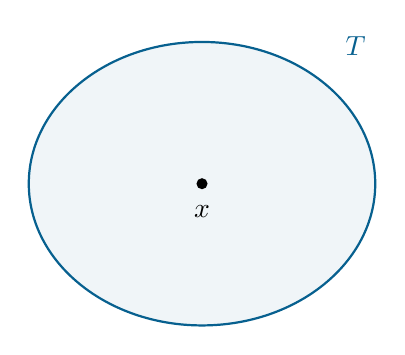
\begin{tikzpicture}
    % (1) Set T
    \fill[figBlue!6] (1.8, 0) ellipse (2.2 and 1.8);
    \draw[thick, figBlue] (1.8, 0) ellipse (2.2 and 1.8);

    % (2) Element x in T
    \fill (1.8, 0) circle (2pt);

    % (3) Text last
    \node[anchor=north] at (1.8, -0.15) {$x$};
    \node[anchor=south west, figBlue] at (3.5, 1.5) {$T$};
\end{tikzpicture}
\end{center}
\end{content}

\begin{aiNote}[Notation: \texorpdfstring{$\subset$ vs.\ $\subseteq$}{subset vs. subseteq}]
% [PERSISTENT]
Many textbooks write $\subseteq$ for an arbitrary (not necessarily proper) subset. In this lecture, the symbol $\subset$ is written for any subset relation ($\operatorname{Stab}(x) \subset G$ and $\operatorname{Orb}(x) \subset T$), without implying strict inclusion.
\end{aiNote}

\begin{speech}[00:18:47 - 00:20:19]
So, the first lemma is that $\operatorname{Stab}(x)$ in $G$ is a subgroup \inlinemetanote{writes: Lemma: $\operatorname{Stab}(x) \subset G$ is subgrp}. And there's nothing to the proof of this, again. It's always, you know... Proof is: there's nothing to it, nothing almost \inlinemetanote{writes: Proof: Nothing.}.

We can check it, though. You need to check, for example, that $e$ is in $\operatorname{Stab}(x)$, so then we have to check that $e \cdot x$ is equal to $x$, but that's condition \textbf{(i)} of the group action \inlinemetanote{writes: $e \in \operatorname{Stab}(x) \Leftarrow e \cdot x = x$ \textbf{(i)}}.

The other one you have to check is if $g_1$ and $g_2$ are in $\operatorname{Stab}(x)$, you have to check that $g_1$ times $g_2$ is in $\operatorname{Stab}(x)$ \inlinemetanote{writes \qt{$g_1, g_2 \in \operatorname{Stab}(x)$} and \qt{$g_1 g_2 \in \operatorname{Stab}(x)$}}. Let's try to do that. We have to figure out what happens when I take this and apply it to $x$ \inlinemetanote{writes: $(g_1 g_2) \cdot x =$}.

So, what do we use here? Well, we have to use some property --- we'll use property \textbf{(ii)}, associativity, which says that exactly this thing is $g_1 (g_2 x)$ \inlinemetanote{writes \qt{$g_1 \cdot (g_2 \cdot x)$} and \textbf{(ii)} by the equals sign}. Okay? And then since this (i.e., $g_2 \cdot x$) is in the stabilizer (i.e., $g_2 \in \operatorname{Stab}(x)$, so $g_2 \cdot x = x$), this is equal to $g_1 \cdot x$, and since $g_1$'s in the stabilizer, this is $x$ \inlinemetanote{writes \qt{$= g_1 \cdot x$} and \qt{$= x$} underneath}. So, we checked it.

And you also have to check the inverse thing, which I leave to you, but they're all checked the same. There's essentially nothing to do in this proof; you just follow. So, that's good.
\end{speech}

\begin{content}[Stabilizer as a Subgroup]
\begin{lemma}[The Stabilizer Is a Subgroup]\label[lemma]{lem:stab-is-subgroup}
For every $x \in T$, $\operatorname{Stab}(x) \subset G$ is a subgroup of $G$.
\end{lemma}

\begin{proof}
We verify the subgroup axioms for $\operatorname{Stab}(x)$:

\textbf{Identity:} We need $e \in \operatorname{Stab}(x)$, which holds because $e \cdot x = x$ by axiom \textbf{(i)} of a group action.

\textbf{Closure under multiplication:} Let $g_1, g_2 \in \operatorname{Stab}(x)$, so that $g_1 \cdot x = x$ and $g_2 \cdot x = x$. To check that $g_1 g_2 \in \operatorname{Stab}(x)$, we apply $g_1 g_2$ to $x$ using axiom \textbf{(ii)} (associativity of the group action):
\begin{align*}
    (g_1 g_2) \cdot x &= g_1 \cdot (g_2 \cdot x) && \text{(by axiom \textbf{(ii)})} \\
    &= g_1 \cdot x && \text{(since $g_2 \in \operatorname{Stab}(x)$)} \\
    &= x && \text{(since $g_1 \in \operatorname{Stab}(x)$).}
\end{align*}
Thus, $g_1 g_2 \in \operatorname{Stab}(x)$.

\textbf{Closure under inverses:} Left to the reader (verified analogously).
\end{proof}

\begin{proof}[Verification of Inverse Closure (beyond the lecture)]
Let $g \in \operatorname{Stab}(x)$, so $g \cdot x = x$. Applying $g^{-1}$ to both sides and using the group action axioms \textbf{(i)} and \textbf{(ii)} yields:
\[
g^{-1} \cdot x = g^{-1} \cdot (g \cdot x) = (g^{-1} g) \cdot x = e \cdot x = x.
\]
Hence, $g^{-1} \in \operatorname{Stab}(x)$.
\end{proof}
\end{content}

\begin{hidden}
% timestamp: 00:20:19
% topic: Stabilizer definition and proof that Stab(x) is a subgroup of G
% board_state: def:stabilizer, lem:stab-is-subgroup
% next_goal: Show that Orb(x) is G-invariant and begin relating G, Orb(x), and Stab(x) via maps
% open_loops: inverse closure of Stab(x) left to students (proved in marked sub-proof)
\end{hidden}

\subsection{\texorpdfstring{$G$}{G}-Invariance of Orbits}

\begin{speech}[00:20:19 - 00:22:37]
So, as I said, this $\operatorname{Orb}(x)$ inside here (i.e., $T$) --- this is a subset \inlinemetanote{writes \qt{$\operatorname{Orb}(x) \subset T$} with \qt{subset} below $\subset$}. There's no notion of being a subgroup here or anything, but it has one property, which is that the $G$-action --- $G$ acts like this \inlinemetanote{writes: $G \times T \to T$}, right?

We could wonder what happens if I try to see what happens on $\operatorname{Orb}$. $G \times T$ maps to $T$ --- that's the action. So, we could see what happens when I put $G$ here and $\operatorname{Orb}$ here \inlinemetanote{writes: $G \times \operatorname{Orb}(x)$}. If we pick a random set, it could go anywhere in $T$, right? But what actually happens is it stays in $\operatorname{Orb}$ \inlinemetanote{completes the arrow: $G \times \operatorname{Orb}(x) \to \operatorname{Orb}(x)$}.

All right? If I take the restriction of the group action, it actually takes $\operatorname{Orb}$ to $\operatorname{Orb}$ \inlinemetanote{writes the restriction symbol $\varphi\big|$ to the left of $G \times \operatorname{Orb}(x)$}. Okay? In this sense, it has a special structure: it's not a random subset of $T$; you could say it's a $G$-invariant subset, it's a subset which respects the $G$-action.

And why is this? Let's check this. This is a claim: it says that if I take $g$ and I take an element in $\operatorname{Orb}$ --- an element in $\operatorname{Orb}$ is something like that \inlinemetanote{writes $g \cdot (h \cdot x)$, with \qt{$\in G$} under $g$ and \qt{$\in \operatorname{Orb}(x)$} under $(h \cdot x)$}. It's some element of the group times $x$. This is an arbitrary element in $G$, and this is an arbitrary element in $\operatorname{Orb}$, okay?

And if I want to check this property, I have to check that when I apply $g$ to an element of $\operatorname{Orb}$, I stay in $\operatorname{Orb}$. Let's just try to do it. Well, we're going to get $g \cdot h \cdot x$ \inlinemetanote{writes: $= g \cdot (h \cdot x)$}.

So, what are we going to do? Well, we have to use associativity. There are only two things to do with the group action: you can either use associativity or this trivial property \inlinemetanote{points at axiom \textbf{(i)} on the previous board}. And the trivial property is so trivial, you don't even have to think about it, so pretty much the only thing you can do is apply associativity. This says that it's $g$ times $h$, $x$ \inlinemetanote{writes: $(gh) \cdot x$}. And then this means it's in $\operatorname{Orb}$, because it's some element of $G$ --- that's the group product --- times $x$ \inlinemetanote{writes \qt{$\operatorname{Orb}(x) \ni$} to the left of $(gh) \cdot x$}. Okay?

So, that's the two structures you get: the stabilizer is a subgroup, and the orbit is a subset, but it's a subset that respects this $G$-action. All right, so...
\end{speech}

\begin{content}[The Action Restricted to an Orbit]
Unlike $\operatorname{Stab}(x) \subset G$, the orbit $\operatorname{Orb}(x) \subset T$ is merely a subset of $T$, so it cannot be a subgroup. Nevertheless, restricting the group action $G \times T \to T$ to $\operatorname{Orb}(x)$ stays inside $\operatorname{Orb}(x)$:
\[
\text{res.}\ G \times \operatorname{Orb}(x) \to \operatorname{Orb}(x).
\]

\begin{claim}[\texorpdfstring{$G$}{G}-Invariance of Orbits]\label[claim]{clm:orbit-g-invariant}
For any $x \in T$, $\operatorname{Orb}(x) \subset T$ is a \newterm{$G$-invariant} subset of $T$: for every $g \in G$ and every $y \in \operatorname{Orb}(x)$, we have
\[
g \cdot y \in \operatorname{Orb}(x).
\]
\end{claim}

\begin{proof}
Let $g \in G$ be an arbitrary group element and let $y = h \cdot x \in \operatorname{Orb}(x)$ (with $h \in G$) be an arbitrary element of the orbit. Acting on $h \cdot x$ by $g$ and applying the associativity axiom \textbf{(ii)} gives:
\[
\underbrace{g}_{\in G} \cdot \underbrace{(h \cdot x)}_{\in \operatorname{Orb}(x)} = g \cdot (h \cdot x) = (gh) \cdot x \in \operatorname{Orb}(x),
\]
since $gh \in G$ by closure of the group operation. (Equivalently, $\operatorname{Orb}(x) \ni (gh) \cdot x$.)
\end{proof}

\begin{steps}[Summary of the Two Structures]
Every group action $G \curvearrowright T$ and choice of $x \in T$ produces two structured subsets:
\begin{itemize}
    \item $\operatorname{Stab}(x) \subset G$ is a \emph{subgroup} of $G$ (\cref{lem:stab-is-subgroup}).
    \item $\operatorname{Orb}(x) \subset T$ is a \emph{$G$-invariant subset} of $T$ (\cref{clm:orbit-g-invariant}), so $G$ restricts to a well-defined action on $\operatorname{Orb}(x)$ itself.
\end{itemize}
\end{steps}
\end{content}

\subsection{Connecting \texorpdfstring{$G$}{G}, Orbits, and Stabilizers}

\begin{speech}[00:22:37 - 00:24:48]
Okay, so then we can put some of these things together with some maps \inlinemetanote{raises the lower-left chalkboard}. Here we have $G$ \inlinemetanote{writes: $G$}.

And the picture is always: we have this $T$ here, and $G$'s acting on $T$, and we have a particular element $x$, and we have this orbit \inlinemetanote{draws a closed contour $T$ below $G$ with an arrow from $G$ to $T$, a point $x$ inside a region of $T$, and shades the region}. Okay, that's what we're concentrating on here: the country $x$'s in, which is the orbit.

So, one map I've already written: we had $A$ goes to $\operatorname{Orb}(x)$ \inlinemetanote{writes: $G \xrightarrow{A} \operatorname{Orb}(x)$}. And this map $A$ takes $g$ to $g$ times $x$ \inlinemetanote{writes: $A\colon g \mapsto g \cdot x$}, okay?

Now we also have the stabilizer, and since the stabilizer's a subgroup, I can consider $G$ mod $\operatorname{Stab}(x)$ \inlinemetanote{writes $\faktor{G}{\operatorname{Stab}(x)}$ above $G \xrightarrow{A} \operatorname{Orb}(x)$}. And I don't know whether it's a normal subgroup. So, by here I mean the set of left cosets. This is the set of left cosets, okay? Do I have to write that?

This is the standard confusion, when, you know... I have not asserted this is a normal subgroup, so I'm not asserting that this quotient is a group, but it is nevertheless a set of cosets; that's what this is. Maybe I write that here \inlinemetanote{writes \qt{set of left cosets} at the upper left and draws an arrow pointing to $\faktor{G}{\operatorname{Stab}(x)}$}.

Okay? And there's a map here, which I call $B$ \inlinemetanote{draws an arrow labeled $B$ from $G$ to $\faktor{G}{\operatorname{Stab}(x)}$}. This map $B$ takes an element $g$ here \inlinemetanote{points at $G$} to $g$ times $\operatorname{Stab}$ \inlinemetanote{writes $g \mapsto g \cdot \operatorname{Stab}(x)$ beside the $B$ arrow} --- takes an element to the left coset. All right?

Maybe, since I don't want to get too crowded there... \inlinemetanote{moves to the right side of the lower-left board} $B$ maps $G$ to $G$ mod $\operatorname{Stab}(x)$ \inlinemetanote{writes: $B \colon G \to \faktor{G}{\operatorname{Stab}(x)}$}. $A$ maps $G$ to $\operatorname{Orb}(x)$ \inlinemetanote{writes: $A \colon G \to \operatorname{Orb}(x)$}. And this takes $g$ to $g$ times $\operatorname{Stab}(x)$, which just takes an element here to that coset, to that equivalence class \inlinemetanote{writes $g \mapsto g \cdot \operatorname{Stab}(x)$ above $B \colon G \to \faktor{G}{\operatorname{Stab}(x)}$}. And this thing here takes $g$ to $g$ times $x$ \inlinemetanote{writes $g \mapsto g \cdot x$ below $A \colon G \to \operatorname{Orb}(x)$}. Is that clear?
\end{speech}

\begin{content}[The Maps \texorpdfstring{$A$}{A} and \texorpdfstring{$B$}{B}]
Fix $x \in T$. Focusing on the orbit $\operatorname{Orb}(x)$ inside $T$ under the action $G \curvearrowright T$:

\definecolor{figBlue}{HTML}{07608F} % RGB (7, 96, 143): petrol blue (MidnightBlue)
\definecolor{figGray}{HTML}{666665} % RGB (102, 102, 101): dark gray (gray!80!black)
\definecolor{figLightGray}{HTML}{A6A6A6} % RGB (166, 166, 166): light gray (gray!70)
\begin{hidden}
- Canvas: no scale, cm; x in [-0.6, 5.75], y in [-2.0, 2.8]
- Order: (1) light fill of T; (2) shaded oval Orb(x) inside T; (3) outlines of Orb(x) and T;
  (4) action arrow from G to T and pointer arrow to Orb(x); (5) point x; (6) all text last
- Coordinates: T = ellipse centre (1.8, 0), radii 2.4 and 2.0 (x in [-0.6, 4.2], y in [-2.0, 2.0]).
  Orb(x) = ellipse centre (1.6, 0.2), radii 1.4 and 0.85 (x in [0.2, 3.0], y in [-0.65, 1.05]).
  Point x at (1.4, 0.2).
  G at (-0.1, 2.45); action arrow from (0.15, 2.45) to (0.55, 1.82) via out=5, in=115 (T's top at x = 0.55 is 1.71).
  Pointer arrow to Orb(x) from (4.5, 0.2) to (2.85, 0.2).
- Labels (normal size, 0.20 per character, height 0.45):
  "G" anchor east at (0.05, 2.45): x in [-0.2, 0.05], y in [2.23, 2.67]
  "T" anchor south west at (3.6, 1.55): T's right edge at y = 1.55 is 3.32
  "x" anchor west at (1.55, 0.2): x in [1.55, 1.8], y in [-0.02, 0.42]
  "\operatorname{Orb}(x)" anchor west at (4.55, 0.2): x in [4.55, 5.75], y in [-0.02, 0.42]
- Collisions: "G" is 0.45 above T; "T" is 0.28 right of outline; "x" inside Orb(x); "\operatorname{Orb}(x)" 0.36 right of T.
\end{hidden}
\begin{center}
\begin{tikzpicture}[>=Stealth]
    % (1) Base fill of T
    \fill[figGray!5] (1.8, 0) ellipse (2.4 and 2.0);

    % (2) Shaded orbit region inside T
    \fill[figBlue!14] (1.6, 0.2) ellipse (1.4 and 0.85);

    % (3) Outlines of Orb(x) and T
    \draw[thick, figBlue] (1.6, 0.2) ellipse (1.4 and 0.85);
    \draw[thick, figBlue] (1.8, 0) ellipse (2.4 and 2.0);

    % (4) Action arrow and pointer arrow
    \draw[->, thick] (0.15, 2.45) to[out=5, in=115] (0.55, 1.82);
    \draw[->, figLightGray] (4.5, 0.2) -- (2.85, 0.2);

    % (5) Point x
    \fill (1.4, 0.2) circle (2pt);

    % (6) Text last
    \node[anchor=east] at (0.05, 2.45) {$G$};
    \node[anchor=south west, figBlue] at (3.6, 1.55) {$T$};
    \node[anchor=west] at (1.55, 0.2) {$x$};
    \node[anchor=west, figBlue] at (4.55, 0.2) {$\operatorname{Orb}(x)$};
\end{tikzpicture}
\end{center}

We now place two canonical maps out of $G$ side by side:
\begin{align*}
    B \colon G &\to \faktor{G}{\operatorname{Stab}(x)}, & g &\mapsto g \cdot \operatorname{Stab}(x), \\
    A \colon G &\to \operatorname{Orb}(x), & g &\mapsto g \cdot x.
\end{align*}

\definecolor{figBlue}{HTML}{07608F} % RGB (7, 96, 143): petrol blue (MidnightBlue)
\definecolor{figGray}{HTML}{666665} % RGB (102, 102, 101): dark gray (gray!80!black)
\definecolor{figLightGray}{HTML}{A6A6A6} % RGB (166, 166, 166): light gray (gray!70)
\begin{hidden}
- Canvas: no scale, cm; first box G placed at (0, 0), every other node placed relative to G or Cosets
- Boxes: name | lines | w x h (cm) | placed
  G      | 1, "$G$" (1 char, 0.2)                      | 0.8 x 0.75 | first, at (0, 0)
  Orb    | 1, "$\operatorname{Orb}(x)$" (6 chars, 1.2) | 1.8 x 0.75 | right=4.8cm of G
  Cosets | 1, "$\faktor{G}{\operatorname{Stab}(x)}$" (7 chars, 1.4, tall 0.7) | 2.0 x 1.0 | above right=2.4cm and 2.2cm of G
  note   | 1, "set of left cosets" (18 chars at \small = 3.24) | 3.8 x 0.75 | left=1.2cm of Cosets
- Coordinates: G centre (0, 0), Orb centre (6.1, 0), Cosets centre (3.6, 2.9 + 0.375) = (3.6, 3.275).
  G spans x in [-0.4, 0.4], y in [-0.375, 0.375].
  Orb spans x in [5.2, 7.0], y in [-0.375, 0.375].
  Cosets spans x in [2.6, 4.6], y in [2.775, 3.775].
  note spans x in [-2.4, 1.4], y in [2.90, 3.65].
- Gaps: G-Orb 4.8; Cosets-note 1.2; note-G (vertically) 2.52.
- Arrows and labels:
  Arrow A from G.east (0.4, 0) to Orb.west (5.2, 0), length 4.8.
  Midpoint Amid = (2.8, 0). "A" above=0.15cm of Amid: y in [0.15, 0.60].
  "A\colon g \mapsto g \cdot x" (10 chars at \small, 1.8) below=0.15cm of Amid: x in [1.9, 3.7], y in [-0.60, -0.15].
  Arrow B from G.north east (0.4, 0.375) to Cosets.south west (2.6, 2.775), length sqrt(2.2^2 + 2.4^2) = 3.26.
  Midpoint Bmid = (1.5, 1.575).
  "B" anchor north west 0.15 below-right of Bmid, at (1.65, 1.425).
  "g \mapsto g \cdot \operatorname{Stab}(x)" (12 chars at \small, 2.16) anchor south east 0.15 above-left of Bmid,
  at (1.35, 1.725): ends below y = 2.20, 0.70 below note (y in [2.90, 3.65]).
- Collisions: note is 1.2 left of Cosets (connected by thin pointer arrow); arrow labels sit on opposite sides of B
  (above-left and below-right) and opposite sides of A (above and below), all >= 0.15 from arrows and >= 0.70 from boxes.
\end{hidden}
\begin{center}
\begin{tikzpicture}[>=Stealth]
    % (1) Text nodes placed via positioning library (first node at origin)
    \node[minimum width=0.8cm, minimum height=0.75cm] (G) at (0, 0) {$G$};
    \node[minimum width=1.8cm, minimum height=0.75cm, right=4.8cm of G] (Orb) {$\operatorname{Orb}(x)$};
    \node[minimum width=2.0cm, minimum height=1.0cm, above right=2.4cm and 2.2cm of G] (Cosets) {$\faktor{G}{\operatorname{Stab}(x)}$};
    \node[minimum width=3.8cm, minimum height=0.75cm, left=1.2cm of Cosets, font=\small, figGray] (note) {set of left cosets};

    % (2) Mapping arrows and pointer arrow
    \draw[->, thick] (G.east) -- coordinate[midway] (Amid) (Orb.west);
    \draw[->, thick, figBlue] (G.north east) -- coordinate[midway] (Bmid) (Cosets.south west);
    \draw[->, figLightGray] (note.east) -- (Cosets.west);

    % (3) Arrow labels last
    \node[anchor=south, yshift=0.15cm] at (Amid) {$A$};
    \node[anchor=north, yshift=-0.15cm, font=\small] at (Amid) {$A\colon g \mapsto g \cdot x$};
    \node[anchor=north west, xshift=0.15cm, yshift=-0.15cm, figBlue] at (Bmid) {$B$};
    \node[anchor=south east, xshift=-0.15cm, yshift=0.15cm, font=\small, figBlue] at (Bmid) {$g \mapsto g \cdot \operatorname{Stab}(x)$};
\end{tikzpicture}
\end{center}

\begin{steps}[Why \texorpdfstring{$\faktor{G}{\operatorname{Stab}(x)}$}{G / Stab(x)} Is Only a Set Here]
Because $\operatorname{Stab}(x) \subset G$ is guaranteed to be a subgroup (\cref{lem:stab-is-subgroup}) but need not be a \emph{normal} subgroup of $G$, the quotient $\faktor{G}{\operatorname{Stab}(x)}$ does not carry a group structure in general. It is, however, always well-defined as the \emph{set of left cosets} $g \cdot \operatorname{Stab}(x)$ for $g \in G$, and $B$ is the canonical quotient projection sending each group element to its left coset.
\end{steps}
\end{content}

\subsection{The Canonical Bijection \texorpdfstring{$C \colon \faktor{G}{\operatorname{Stab}(x)} \to \operatorname{Orb}(x)$}{C: G / Stab(x) -> Orb(x)}}

\begin{speech}[00:24:48 - 00:25:53]
All right, and so then the first part of this Orbit--Stabilizer Theorem says that there exists a map $C$ --- $A, B, C$ \inlinemetanote{writes: $\exists\, C \colon \faktor{G}{\operatorname{Stab}(x)} \to \operatorname{Orb}(x)$}. And where's this map going to go? It's going to go $G$ mod $\operatorname{Stab}(x)$ to $\operatorname{Orb}(x)$, okay?

So, I first have to define it. The definition is that $C$ --- so what does $C$ eat? It's one of these equivalence classes \inlinemetanote{points at $\faktor{G}{\operatorname{Stab}(x)}$}. I have to define it, I have to feed it an equivalence class \inlinemetanote{writes: $\text{Def}\colon C(g \cdot \operatorname{Stab}(x)) =$}. Okay? And it returns an element of the orbit.

What element of the orbit do you think it's going to return? This is kind of a linguistic question because you have to complete this. What do you think? It should be an element of the orbit, so it should be $x$ times something, 'cause that's what an element of the orbit is \inlinemetanote{writes $x$ on the right-hand side}. And $x$ times what? Yeah?
\end{speech}

\begin{student}[Student Answer]
Times, like, there's some sort of combination of $g$ and $h$?
\end{student}

\begin{speech}[00:25:56 - 00:25:58]
But what --- there's no $h$ on the board.
\end{speech}

\begin{student}[Student Answer, continued]
Oh, right, just $g$.
\end{student}

\begin{speech}[00:26:00 - 00:26:42]
Okay, yeah, this is the solid answer, because there's nothing else on the board \inlinemetanote{writes $g \cdot$ in front of $x$}. I submit there's nothing else you could write here. Because if you want to define a map from here to the orb \inlinemetanote{points at $\faktor{G}{\operatorname{Stab}(x)} \to \operatorname{Orb}(x)$}, the only data you have here is this \inlinemetanote{points at $g \cdot \operatorname{Stab}(x)$}, and you have to produce an element in the orbit, so it should be $x$ times something --- it's $g$.

But this is a proposal of a definition for the usual reasons, because we have to check what happens \inlinemetanote{writes \qt{Proposal} above the equals sign}. So, we have to check the standard stuff: Check, is this well-defined \inlinemetanote{writes: Check: is this well-defined?}?
\end{speech}

\begin{content}[Proposed Definition of \texorpdfstring{$C$}{C}]
We seek a map
\[
\exists\, C \colon \faktor{G}{\operatorname{Stab}(x)} \to \operatorname{Orb}(x).
\]
Given a left coset $g \cdot \operatorname{Stab}(x) \in \faktor{G}{\operatorname{Stab}(x)}$, the natural candidate definition is:
\[
C\bigl(g \cdot \operatorname{Stab}(x)\bigr) \stackrel{\text{Proposal}}{=} g \cdot x.
\]

\begin{question}\label[question]{q:c-well-defined}
Is the proposed map $C\bigl(g \cdot \operatorname{Stab}(x)\bigr) = g \cdot x$ well-defined?
\end{question}

\begin{steps}[Why Well-Definedness Must Be Checked]
A left coset $g \cdot \operatorname{Stab}(x)$ is an equivalence class of group elements, so it can have many different representatives ($g$ and $\hat{g}$ with $g \cdot \operatorname{Stab}(x) = \hat{g} \cdot \operatorname{Stab}(x)$). Because the proposed formula $g \cdot x$ uses the chosen representative $g$, we must verify that choosing a different representative $\hat{g}$ of the same coset yields the exact same element in $\operatorname{Orb}(x)$.
\end{steps}
\end{content}

\begin{hidden}
% timestamp: 00:07:35
% topic: Definition proposal for C: G / Stab(x) -> Orb(x)
% board_state: q:c-well-defined, lem:stab-is-subgroup, clm:orbit-g-invariant
% next_goal: Verify that C is well-defined, surjective, and injective, then state the Orbit--Stabilizer Theorem
% open_loops: q:c-well-defined
\end{hidden}

\begin{speech}[00:26:42 - 00:28:49]
So, let's try to check it. Suppose we have $C$ of $g$ times $\operatorname{Stab}(x)$ \inlinemetanote{writes: $C(g \cdot \operatorname{Stab}(x))$}. Is this equal, under this proposal, to $C$ of $\hat{g}$ times $\operatorname{Stab}(x)$ \inlinemetanote{writes: $\stackrel{?}{=} C(\hat{g} \cdot \operatorname{Stab}(x))$}, because it's this usual naming problem: this is a coset, it's an equivalence class, it has many names?

Well, let's try to check. So, this side, this would be $g$ times $x$, and this side here is $\hat{g}$ times $x$ \inlinemetanote{writes $g \cdot x$ beneath $C(g \cdot \operatorname{Stab}(x))$ and $\hat{g} \cdot x$ beneath $C(\hat{g} \cdot \operatorname{Stab}(x))$}. But what's the assumption? We check this under the assumption that $g \operatorname{Stab}(x)$ equals $\hat{g} \operatorname{Stab}(x)$ \inlinemetanote{writes: Under $g \cdot \operatorname{Stab}(x) = \hat{g} \cdot \operatorname{Stab}(x)$}. That means we take two cosets, they're the same, take two different representatives, we get two things \inlinemetanote{points at $g \cdot x$ and $\hat{g} \cdot x$}, and the question is: are these the same? So, the question about \qt{well-defined} is: is this the same \inlinemetanote{writes $\stackrel{?}{=}$ between $g \cdot x$ and $\hat{g} \cdot x$}?

We have to see: well, what this means is that $\hat{g}$ is equal to $g$ times something \inlinemetanote{writes: $\hat{g} = g \cdot s$}. Because $\hat{g}$ is here (in $\hat{g} \cdot \operatorname{Stab}(x)$), and if it's in that equivalence class, $\hat{g}$'s something times something, where the something --- I'll try to write my $s$'s here cursive --- $s$ is in the stabilizer \inlinemetanote{writes: $s \in \operatorname{Stab}(x)$}.

Okay, then we can check: $\hat{g}$ (acting on $x$), this is equal to $g s x$, okay, using this equation \inlinemetanote{points at $\hat{g} = g \cdot s$ and writes \qt{$= g \cdot s \cdot x$}}. But now $s$ is in the stabilizer, so when $s$ acts on $x$, it does nothing. So, this is $g x$ \inlinemetanote{writes: $= g \cdot x$}. This $s$ acting on $x$ goes away --- that's how you become an element of the stabilizer. So, the answer is well-defined.

So, are there questions about this? This is the kind of thing we've done probably like half a dozen times in this class already. It's just always in slightly different context. But it should not surprise you.

That's kind of good news: $C$ is well-defined. \inlinemetanote{raises the lower-middle board}
\end{speech}

\begin{content}[Well-Definedness of \texorpdfstring{$C$}{C}]
\begin{answer}[to \cref{q:c-well-defined}]\label[answer]{ans:c-well-defined}
Yes, the map $C \colon \faktor{G}{\operatorname{Stab}(x)} \to \operatorname{Orb}(x)$ given by $C\bigl(g \cdot \operatorname{Stab}(x)\bigr) := g \cdot x$ is well-defined.
\end{answer}

\begin{claim}[Well-Definedness of \texorpdfstring{$C$}{C}]\label[claim]{clm:c-well-defined}
If $g, \hat{g} \in G$ satisfy $g \cdot \operatorname{Stab}(x) = \hat{g} \cdot \operatorname{Stab}(x)$, then $g \cdot x = \hat{g} \cdot x$.
\end{claim}

\begin{proof}
Suppose $g \cdot \operatorname{Stab}(x) = \hat{g} \cdot \operatorname{Stab}(x)$. Since $\hat{g} = \hat{g} \cdot e \in \hat{g} \cdot \operatorname{Stab}(x)$, we have $\hat{g} \in g \cdot \operatorname{Stab}(x)$, which means there exists an element $s \in \operatorname{Stab}(x)$ such that:
\[
\hat{g} = g \cdot s.
\]
Comparing the proposed values for the two representatives $\hat{g}$ and $g$, we compute:
\begin{align*}
    \hat{g} \cdot x &= (g \cdot s) \cdot x && \text{(since $\hat{g} = g \cdot s$)} \\
    &= g \cdot (s \cdot x) && \text{(by associativity of the action)} \\
    &= g \cdot x && \text{(since $s \in \operatorname{Stab}(x)$, so $s \cdot x = x$).}
\end{align*}
Hence, the proposed value $g \cdot x$ does not depend on the choice of coset representative, so $C$ is well-defined.
\end{proof}
\end{content}

\begin{speech}[00:28:49 - 00:30:04]
Is $C$ surjective? \inlinemetanote{erases the lower-left chalkboard} Oh, yeah, the other language I speak is Portuguese, by the way.

Okay, so, we have $C$ is well-defined. Now, is $C$ surjective \inlinemetanote{writes: Is $C$ surjective?}?

So, what's the answer to that? Well, $C$, you see, you put in any equivalence class, you get $g(x)$ (i.e., $g \cdot x$), but $g \cdot x$ reflects every single element of the orbit, right? 'Cause that's the way: an arbitrary element of an orbit is $x$ pushed around by some $g$. So, it's just surjective by definition.

Is $C$ surjective? And that's yes, by definition \inlinemetanote{writes: Yes, by definition.}. Is that clear? It's just --- you know, what was the definition of the orbit? It's those things that you get by pushing $x$ around by some group element. And whatever the group element of that is, you can make it in the equivalence class and go to that \inlinemetanote{points along the diagram arrows from $G$ through $\faktor{G}{\operatorname{Stab}(x)}$ to $\operatorname{Orb}(x)$}. So, it's actually just by definition it's surjective. It's not really a mathematical statement; it's just by definition.
\end{speech}

\begin{content}[Surjectivity of \texorpdfstring{$C$}{C}]
\begin{claim}[Surjectivity of \texorpdfstring{$C$}{C}]\label[claim]{clm:c-surjective}
The map $C \colon \faktor{G}{\operatorname{Stab}(x)} \to \operatorname{Orb}(x)$ is surjective.
\end{claim}

\begin{proof}
By definition, any element $y \in \operatorname{Orb}(x)$ is of the form $y = g \cdot x$ for some $g \in G$ (\cref{def:orbit}). Taking the left coset $g \cdot \operatorname{Stab}(x) \in \faktor{G}{\operatorname{Stab}(x)}$ gives $C\bigl(g \cdot \operatorname{Stab}(x)\bigr) = g \cdot x = y$.
\end{proof}
\end{content}

\begin{speech}[00:30:04 - 00:31:04]
Now, what about: is $C$ injective \inlinemetanote{writes: Is $C$ injective?}?

So, let's try to check about this. That has to do with: if I take $C$ of $g$ $\operatorname{Stab}(x)$ --- this is one equivalence class --- and suppose it equals $C$ of another equivalence class \inlinemetanote{writes \qt{$C(g \cdot \operatorname{Stab}(x))$} and \qt{$= C(\hat{g} \cdot \operatorname{Stab}(x))$}}. By definition, this is $g$ of $x$ (i.e., $g \cdot x$), and then this is $\hat{g}$ of $x$ (i.e., $\hat{g} \cdot x$) \inlinemetanote{writes $g \cdot x$ beneath $C(g \cdot \operatorname{Stab}(x))$ and $\hat{g} \cdot x$ beneath $C(\hat{g} \cdot \operatorname{Stab}(x))$}. And these things are equal.

If $C$ of somebody is equal, then we get the equation $gx = \hat{g}x$, and this equation is in $T$ \inlinemetanote{writes: We get $g \cdot x = \hat{g} \cdot x \in T$}.

What do you think we should do here? \inlinemetanote{pauses for a response from the class} Yeah?
\end{speech}

\begin{student}[Student Answer]
Like, multiply with $\hat{g}$ inverse?
\end{student}

\begin{speech}[00:31:07 - 00:32:51]
Or $g$ inverse, yeah, let's try that. So, if we multiply with $g$ inverse, we get $x = g^{-1} \hat{g} x$ \inlinemetanote{writes: $x = g^{-1} \hat{g} x$}. That's just... these are elements of $T$, so I can act with any element of $G$ on top of this, and I act with $g^{-1}$. When I act with $g^{-1}$, these things cancel out and the $g^{-1}$ is over there.

Okay, and what do we deduce from this? Well, we deduce --- which is what you're going to say next --- that $g^{-1} \hat{g}$ is in the stabilizer \inlinemetanote{writes: We deduce $g^{-1} \hat{g} \in \operatorname{Stab}(x)$}. 'Cause that's the definition --- that's the ticket to being in the stabilizer of $x$, is when you act on $x$ you don't do anything.

So, that means that $g^{-1} \hat{g}$ is equal to $s$, where $s$ is in the stabilizer \inlinemetanote{writes: $g^{-1} \hat{g} = s \in \operatorname{Stab}(x)$}. And so, the conclusion is: multiply now --- we undo it: this is an element in the group, so we multiply by $g$ on both sides. If we multiply by $g$ on both sides, we get $\hat{g}$ is equal to $gs$, and this is an equation in the group \inlinemetanote{writes: $\hat{g} = g s, \in G$}.

And this shows that... that says that the equivalence classes are the same; that's what it means --- this means that $\hat{g}$ was in this equivalence class. So, this implies that $g \operatorname{Stab}(x) = \hat{g} \operatorname{Stab}(x)$ in the set of equivalence classes \inlinemetanote{writes: $\implies g \cdot \operatorname{Stab}(x) = \hat{g} \cdot \operatorname{Stab}(x) \in \faktor{G}{\operatorname{Stab}(x)}$}.

Okay, so, that's great! Not only did we define $C$, not only is it well-defined, it's injective and surjective, so it's bijective. Yeah?
\end{speech}

\begin{content}[Injectivity of \texorpdfstring{$C$}{C}]
\begin{claim}[Injectivity of \texorpdfstring{$C$}{C}]\label[claim]{clm:c-injective}
The map $C \colon \faktor{G}{\operatorname{Stab}(x)} \to \operatorname{Orb}(x)$ is injective.
\end{claim}

\begin{proof}
Suppose that two left cosets have the same image under $C$:
\[
C\bigl(g \cdot \operatorname{Stab}(x)\bigr) = C\bigl(\hat{g} \cdot \operatorname{Stab}(x)\bigr).
\]
By definition of $C$, this gives the equality in $T$:
\[
g \cdot x = \hat{g} \cdot x \in T.
\]
Since $g \cdot x$ and $\hat{g} \cdot x$ are elements of $T$, we may act on both sides by $g^{-1} \in G$. Using the group action axioms \textbf{(i)} and \textbf{(ii)}:
\[
x = e \cdot x = (g^{-1} g) \cdot x = g^{-1} \cdot (g \cdot x) = g^{-1} \cdot (\hat{g} \cdot x) = (g^{-1} \hat{g}) \cdot x.
\]
Hence, $x = (g^{-1} \hat{g}) \cdot x$, from which we deduce by \cref{def:stabilizer} that
\[
g^{-1} \hat{g} \in \operatorname{Stab}(x).
\]
Writing $g^{-1} \hat{g} = s$ for some $s \in \operatorname{Stab}(x)$ and multiplying on the left by $g$ inside the group $G$, we obtain:
\[
\hat{g} = g s \in G.
\]
Because $\hat{g} = g s \in g \cdot \operatorname{Stab}(x)$, the two left cosets coincide:
\[
g \cdot \operatorname{Stab}(x) = \hat{g} \cdot \operatorname{Stab}(x) \in \faktor{G}{\operatorname{Stab}(x)}.
\]
Thus, $C$ is injective. Combining \cref{clm:c-well-defined,clm:c-surjective,clm:c-injective}, $C$ is a bijection.
\end{proof}
\end{content}

\begin{student}[Student Question]
Why can't we just multiply by, uh, $x$ inverse?
\end{student}

\begin{speech}[00:32:54 - 00:33:05]
$x$ you can't multiply --- $x$ is in $T$. Yeah, yeah --- I mean, $T$ is different. Yeah.
\end{speech}

\begin{student}[Student Question]
What's the difference between this proof and that proof?
\end{student}

\begin{speech}[00:33:09 - 00:33:52]
That --- yeah, I mean, we're riding the train in kind of different directions, not so much different.

This is where... here we're trying to find out whether $C$ is well-defined \inlinemetanote{points at the upper-middle board}. So, we take two equivalence classes that we know at the beginning are the same, and then we show that the value of $C$ is the same.

This \inlinemetanote{points at the lower-middle board}, we wanted to prove injectivity, so we take two equivalence classes that we don't know are the same, but their $C$ is the same, and then we deduce that they're the same.

But, I mean, the comment is reasonable; it's like there's one train, and we're riding it one way and then back the other way. It's kind of the same argument in reverse.
\end{speech}

\begin{insight}[Well-Definedness vs.\ Injectivity: \qt{Riding the Train} in Opposite Directions]
Proving well-definedness (\cref{clm:c-well-defined}) and proving injectivity (\cref{clm:c-injective}) are the two reverse directions of the exact same equivalence chain, with $g^{-1}\hat{g} \in \operatorname{Stab}(x)$ as the shared bridge:
\begin{align*}
\text{Well-definedness:} \quad & g \cdot \operatorname{Stab}(x) = \hat{g} \cdot \operatorname{Stab}(x) \implies g^{-1}\hat{g} \in \operatorname{Stab}(x) \implies g \cdot x = \hat{g} \cdot x, \\
\text{Injectivity:} \quad & g \cdot x = \hat{g} \cdot x \implies g^{-1}\hat{g} \in \operatorname{Stab}(x) \implies g \cdot \operatorname{Stab}(x) = \hat{g} \cdot \operatorname{Stab}(x).
\end{align*}
Also note why one cannot \qt{cancel $x$}: $x$ lives in the set $T$, which has no group multiplication or inverses --- only elements of $G$ (such as $g^{-1}$) can act on both sides of $g \cdot x = \hat{g} \cdot x$.
\end{insight}

\begin{hidden}
% timestamp: 00:14:45
% topic: Well-definedness, surjectivity, and injectivity of C verified; student Q&A resolved
% board_state: clm:c-well-defined, clm:c-surjective, clm:c-injective
% next_goal: Formally state the Orbit--Stabilizer Theorem with commutative diagrams
% open_loops: none
\end{hidden}

\subsection{Statement of the Orbit--Stabilizer Theorem}

\begin{speech}[00:33:52 - 00:34:58]
Okay, so now we can state the Orbit--Stabilizer Theorem in the first version. \inlinemetanote{raises the lower boards up and erases the boards moved down to clear fresh space}

But, as always in this class, I mean, all the definitions are perfect, so, you know, everything just works. You have to allow the definitions to prove the theorems; in some sense that's all you have to do. Which, another way of saying it, is: if you understand the definitions correctly, then all of the stuff I'm lecturing here will just prove itself.

I mean, in this discussion of group actions there'll be some non-trivial theorems, like the Sylow theorems, that have additional ideas, but we haven't come to them yet. This is all just exploration of the definitions, basically. Okay, so...
\end{speech}

\begin{speech}[00:34:58 - 00:36:49]
So, we complete the diagram. This Orbit--Stabilizer Theorem is that when we have $G$ acting on $T$ and $x$ in $T$, then we have this picture: $G$ with the map $A$ to $\operatorname{Orb}(x)$, and then we have the map $B$ to $G$ mod $\operatorname{Stab}(x)$, and then the Orbit--Stabilizer Theorem says that there exists a $C$ here, which we've constructed \inlinemetanote{writes \qt{\underline{Orb--Stab Thm:}}, \qt{$G \curvearrowright T$}, \qt{$x \in T$}, and \qt{then:}, and draws the commutative triangle $G \xrightarrow{A} \operatorname{Orb}(x)$, $G \xrightarrow{B} \faktor{G}{\operatorname{Stab}(x)}$, and $\faktor{G}{\operatorname{Stab}(x)} \xrightarrow{\exists\, C} \operatorname{Orb}(x)$}.

And it has several properties. One is $C$ of the formula I gave; this is a well-defined map \inlinemetanote{writes: $\bullet\; C(g \cdot \operatorname{Stab}(x)) = g \cdot x$}. The second is that $C$ is a bijection \inlinemetanote{writes: $\bullet\; C \text{ is bijection.}$}. And the third is that this diagram commutes \inlinemetanote{writes: $\bullet\; \text{Diagram commutes}$}. Do you know that terminology? This is kind of standard math terminology: the diagram commutes, meaning that you can take $G$, you can go here (to $\faktor{G}{\operatorname{Stab}(x)}$) and go by $C$, or you can go straight to $A$ (i.e., along $A$ to $\operatorname{Orb}(x)$), and the answer's the same.

And the last one is if you take $g$, and if you go up, that's $g$ times $\operatorname{Stab}(x)$, and then if this is by $B$, if you go then by $C$, the answer, by the definition of $C$, is $g$ times $x$, and that's the same as just going over here \inlinemetanote{draws the element-level triangle with $g \mapsto g \cdot \operatorname{Stab}(x)$ via $B$, $g \cdot \operatorname{Stab}(x) \mapsto g \cdot x$ via $C$, and $g \mapsto g \cdot x$ via $A$}. So, that's the diagram commuting.

This is the basic aspect of the Orbit--Stabilizer Theorem. There's one more refinement which I'll talk about next time. Yeah.
\end{speech}

\begin{content}
\begin{theorem}[Orbit--Stabilizer Theorem]\label[theorem]{thm:orbit-stabilizer}
Let $G \curvearrowright T$ be a group action and let $x \in T$. Then there exists a map
\[
C \colon \faktor{G}{\operatorname{Stab}(x)} \to \operatorname{Orb}(x)
\]
defined by $C\bigl(g \cdot \operatorname{Stab}(x)\bigr) := g \cdot x$ such that:
\begin{itemize}
    \item $C$ is a well-defined bijection (\cref{clm:c-well-defined,clm:c-surjective,clm:c-injective}), and
    \item the diagram below commutes (i.e., $C \circ B = A$):
\end{itemize}

\definecolor{figBlue}{HTML}{07608F} % RGB (7, 96, 143): petrol blue (MidnightBlue)
\definecolor{figGreen}{HTML}{3D8252} % RGB (61, 130, 82): dark green (ForestGreen!70!black)
\definecolor{figRed}{HTML}{B5251C} % RGB (181, 37, 28): brick red (BrickRed)
\begin{hidden}
- Canvas: no scale, cm; two triangles side by side, placed purely relative to the first node G (left) and g (right)
- Left triangle boxes: name | lines | w x h (cm) | placed
  G      | 1, "$G$"                                    | 0.8 x 0.75 | first, at (0, 0)
  Orb    | 1, "$\operatorname{Orb}(x)$"                | 1.8 x 0.75 | right=4.4cm of G
  Cosets | 1, "$\faktor{G}{\operatorname{Stab}(x)}$"   | 2.0 x 1.0  | above right=2.4cm and 1.2cm of G
- Left triangle positions:
  G in [-0.4, 0.4] x [-0.375, 0.375]; Orb in [4.8, 6.6] x [-0.375, 0.375];
  Cosets south west = (0.4 + 1.2, 0.375 + 2.4) = (1.6, 2.775), so Cosets in [1.6, 3.6] x [2.775, 3.775].
  Arrows:
  A: G.east (0.4, 0) -- Orb.west (4.8, 0), midpoint (2.6, 0). Label "A" above=0.15cm of Amid.
  B: G.north east (0.4, 0.375) -- Cosets.south west (1.6, 2.775), midpoint (1.0, 1.575). Label "B" above left=0.15cm of Bmid.
  \exists C: Cosets.south east (3.6, 2.775) -- Orb.north west (4.8, 0.375), midpoint (4.2, 1.575). Label "\exists C" above right=0.15cm of Cmid.
- Right triangle boxes (element-wise action):
  g     | 1, "$g$"                        | 0.8 x 0.75 | right=2.2cm of Orb (west = 8.8, centre = 9.2)
  gx    | 1, "$g \cdot x$"                | 1.2 x 0.75 | right=3.8cm of g (west = 13.4, east = 14.6)
  gstab | 1, "$g \cdot \operatorname{Stab}(x)$" | 2.6 x 0.75 | above right=2.4cm and 0.8cm of g (south west = (10.4, 2.775), x in [10.4, 13.0], y in [2.775, 3.525])
- Right triangle arrows (|->):
  g.east -- gx.west (A above=0.15cm of amid2), g.north east -- gstab.south west (B above left=0.15cm of bmid2),
  gstab.south east -- gx.north west (C above right=0.15cm of cmid2).
- Gaps: left-to-right triangles 2.2cm between Orb and g; horizontal arrows 4.4 and 3.8 long; all edge labels >= 0.15cm from arrows and >= 0.8cm from boxes.
\end{hidden}
\begin{center}
\begin{tikzpicture}[>=Stealth, scale=0.88, transform shape]
    % Left triangle: maps between sets
    \node[minimum width=0.8cm, minimum height=0.75cm] (G) at (0, 0) {$G$};
    \node[minimum width=1.8cm, minimum height=0.75cm, right=4.4cm of G] (Orb) {$\operatorname{Orb}(x)$};
    \node[minimum width=2.0cm, minimum height=1.0cm, above right=2.4cm and 1.2cm of G] (Cosets) {$\faktor{G}{\operatorname{Stab}(x)}$};

    \draw[->, thick] (G.east) -- coordinate[midway] (Amid) (Orb.west);
    \draw[->, thick, figBlue] (G.north east) -- coordinate[midway] (Bmid) (Cosets.south west);
    \draw[->, thick, figRed] (Cosets.south east) -- coordinate[midway] (Cmid) (Orb.north west);

    \node[above=0.15cm] at (Amid) {$A$};
    \node[above left=0.15cm, figBlue] at (Bmid) {$B$};
    \node[above right=0.15cm, figRed] at (Cmid) {$\exists\, C$};

    % Right triangle: element-wise correspondence
    \node[minimum width=0.8cm, minimum height=0.75cm, right=2.2cm of Orb] (g) {$g$};
    \node[minimum width=1.2cm, minimum height=0.75cm, right=3.8cm of g] (gx) {$g \cdot x$};
    \node[minimum width=2.6cm, minimum height=0.75cm, above right=2.4cm and 0.8cm of g] (gstab) {$g \cdot \operatorname{Stab}(x)$};

    \draw[|->, thick] (g.east) -- coordinate[midway] (amid2) (gx.west);
    \draw[|->, thick, figBlue] (g.north east) -- coordinate[midway] (bmid2) (gstab.south west);
    \draw[|->, thick, figRed] (gstab.south east) -- coordinate[midway] (cmid2) (gx.north west);

    \node[above=0.15cm] at (amid2) {$A$};
    \node[above left=0.15cm, figBlue] at (bmid2) {$B$};
    \node[above right=0.15cm, figRed] at (cmid2) {$C$};
\end{tikzpicture}
\end{center}
\end{theorem}

\begin{steps}[Meaning of Commutativity]
Saying that the diagram \emph{commutes} means that following the two-step path $G \xrightarrow{B} \faktor{G}{\operatorname{Stab}(x)} \xrightarrow{C} \operatorname{Orb}(x)$ produces the exact same result as taking the direct path $G \xrightarrow{A} \operatorname{Orb}(x)$:
\[
(C \circ B)(g) = C\bigl(g \cdot \operatorname{Stab}(x)\bigr) = g \cdot x = A(g) \qquad \forall g \in G.
\]
\end{steps}
\end{content}

\subsection{Consequences for Finite Groups and Finite Sets}

\begin{speech}[00:36:49 - 00:39:35]
So, it has interesting consequences \inlinemetanote{draws a vertical line separating the right side of the lower-right board}. And one of them is: if $G$ --- let's say $G$ and $T$ --- actually, you just need: suppose $G$ is finite, and $T$ can be anything \inlinemetanote{writes: $G \text{ is finite},\; T \text{ anything}$}. Right? So, we have here $T$ --- meaning that $T$ could be finite or infinite \inlinemetanote{draws a closed contour $T$ with curved partition lines and a shaded orbit region containing a dot $x$}.

And if $G$ is finite, then these countries here, the orb \inlinemetanote{points at the shaded orbit region} --- $G$ finite implies, of course, the orbit of $x$ is also finite \inlinemetanote{writes \qt{$G$ finite} with a downward $\implies$ to \qt{$\operatorname{Orb}(x)$ finite}}. Because, if you remember, the way that you get the orbit of $x$ is by pushing around by elements of $G$, so if $G$'s finite, you only have finitely many possibilities.

But this Orbit--Stabilizer Theorem tells you something great, which is it says: what is the size of this orbit \inlinemetanote{writes: $|\operatorname{Orb}(x)| =$ }? The size of the orbit, since this is a bijection \inlinemetanote{points back at the bullet \qt{$C$ is bijection} on the left}, is actually the size of $G$, the number of cosets of the stabilizer \inlinemetanote{writes: $\left|\faktor{G}{\operatorname{Stab}(x)}\right|$}. Okay?

And we've already proven by Lagrange's Theorem that this is a divisor of $G$, the number of elements of $G$. So, as a consequence, the size of the orbit --- it cannot be any number; it has to be some number that divides the order of $G$ \inlinemetanote{writes: $|\operatorname{Orb}(x)| \mid |G|$}.

This is one of the consequences of the Orbit--Stabilizer Theorem: that when you have a finite group, it's spinning around this $T$ in crazy ways, but each orbit --- it's extremely constrained how big that orbit is: it has to be a divisor of $G$ (i.e., $|G|$).

I remind you, though, that there are two divisors which are kind of common: one is that it could be $1$ --- you know, $1$ is always a divisor of $G$, that's always legal --- or it could be all of $G$. Those are sometimes the most common. And in the case of $1$, it has a special name, so let me say that... \inlinemetanote{looks at the remaining boards and walks back toward the middle}

Yes. But this is a very strong constraint. And this is typically how the Orbit--Stabilizer Theorem is used, for this deduction that the size of the orbit has to divide the order of $G$ in the finite case.

I remind you, the Orbit--Stabilizer Theorem is a statement that did not require anybody to be finite. If $G$ and $T$ are infinite, these orbits and the number of cosets could be infinite; that's okay for this theorem. It's just saying $C$ is a bijection, which is an okay statement even if it's infinite.
\end{speech}

\begin{content}[Orbit Sizes When \texorpdfstring{$G$}{G} Is Finite]
\begin{corollary}[Divisibility of Orbit Sizes]\label[corollary]{cor:orbit-divides-group}
Suppose $G$ is a finite group acting on an arbitrary (possibly infinite) set $T$, and let $x \in T$. Then $\operatorname{Orb}(x)$ is finite, its cardinality equals the index of the stabilizer,
\[
|\operatorname{Orb}(x)| = \left|\faktor{G}{\operatorname{Stab}(x)}\right|,
\]
and consequently the size of every orbit divides the order of $G$:
\[
|\operatorname{Orb}(x)| \mid |G|.
\]
\end{corollary}

\definecolor{figBlue}{HTML}{07608F} % RGB (7, 96, 143): petrol blue (MidnightBlue)
\definecolor{figGray}{HTML}{666665} % RGB (102, 102, 101): dark gray (gray!80!black)
\definecolor{figLightGray}{HTML}{A6A6A6} % RGB (166, 166, 166): light gray (gray!70)
\begin{hidden}
- Canvas: no scale, cm; T = ellipse centre (0, 0), radii 2.3 and 1.8 (x in [-2.3, 2.3], y in [-1.8, 1.8]);
  picture spans x in [-2.3, 4.1], y in [-1.8, 1.85]
- Order: (1) light fill of T; (2) shaded orbit band between c1 and c2, clipped to T; (3) partition curves and outline of T;
  (4) pointer arrow to Orb(x); (5) point x; (6) all text last
- Coordinates: curves inside T:
  c1: y = 0.85 + 0.04*x^2
  c2: y = -0.15 + 0.10*sin(90*x)
  c3: y = -0.95 - 0.04*x^2
  Point x at (0.2, 0.35), between c1 (0.85) and c2 (-0.12).
  Pointer arrow for Orb(x) from (2.7, 0.35) to (2.0, 0.35); T's right edge at y = 0.35 is 2.26.
- Labels (normal size, 0.20 per character, height 0.45):
  "T" anchor south west at (1.75, 1.40): T's right edge at y = 1.40 is 1.45, 0.30 left
  "x" anchor west at (0.35, 0.35): x in [0.35, 0.60], y in [0.13, 0.57]
  "\operatorname{Orb}(x)" (6 chars, 1.2) anchor west at (2.75, 0.35): x in [2.75, 3.95], y in [0.13, 0.57]
- Collisions: "x" 0.28 below c1 and 0.25 above c2; "\operatorname{Orb}(x)" 0.49 right of T's edge (2.26); "T" 0.30 right of T.
\end{hidden}
\begin{center}
\begin{tikzpicture}[>=Stealth]
    % (1) Base fill of T
    \fill[figGray!5] (0, 0) ellipse (2.3 and 1.8);

    % (2), (3) Shaded orbit region and partition curves clipped inside T
    \begin{scope}
        \clip (0, 0) ellipse (2.3 and 1.8);
        \fill[figBlue!14]
            plot[domain=-2.3:2.3, samples=50] (\x, {0.85 + 0.04*\x*\x})
            -- plot[domain=2.3:-2.3, samples=50] (\x, {-0.15 + 0.10*sin(90*\x)})
            -- cycle;
        \draw[figGray, domain=-2.3:2.3, samples=50, smooth] plot (\x, {0.85 + 0.04*\x*\x});
        \draw[figGray, domain=-2.3:2.3, samples=50, smooth] plot (\x, {-0.15 + 0.10*sin(90*\x)});
        \draw[figGray, domain=-2.3:2.3, samples=50, smooth] plot (\x, {-0.95 - 0.04*\x*\x});
    \end{scope}
    \draw[thick, figBlue] (0, 0) ellipse (2.3 and 1.8);

    % (4) Pointer arrow to shaded orbit
    \draw[->, figLightGray] (2.7, 0.35) -- (2.0, 0.35);

    % (5) Point x
    \fill (0.2, 0.35) circle (2pt);

    % (6) Text last
    \node[anchor=south west, figBlue] at (1.75, 1.40) {$T$};
    \node[anchor=west] at (0.35, 0.35) {$x$};
    \node[anchor=west, figBlue] at (2.75, 0.35) {$\operatorname{Orb}(x)$};
\end{tikzpicture}
\end{center}

\begin{proof}
Because $G$ is finite and $\operatorname{Orb}(x) = \{ g \cdot x \mid g \in G \}$, $\operatorname{Orb}(x)$ is also finite. By the Orbit--Stabilizer Theorem (\cref{thm:orbit-stabilizer}), $C \colon \faktor{G}{\operatorname{Stab}(x)} \to \operatorname{Orb}(x)$ is a bijection, so
\[
|\operatorname{Orb}(x)| = \left|\faktor{G}{\operatorname{Stab}(x)}\right|.
\]
Since $\operatorname{Stab}(x) \subset G$ is a subgroup (\cref{lem:stab-is-subgroup}), Lagrange's Theorem implies that the number of left cosets $\left|\faktor{G}{\operatorname{Stab}(x)}\right| = [G : \operatorname{Stab}(x)] = \frac{|G|}{|\operatorname{Stab}(x)|}$ divides $|G|$. Hence, $|\operatorname{Orb}(x)| \mid |G|$.
\end{proof}

\begin{steps}[Extreme Cases and Infinite Generality]
\begin{itemize}
    \item \textbf{Common divisors:} Two particularly frequent orbit sizes are $1$ (whose special name is deferred to the next lecture) and $|G|$.
    \item \textbf{No finiteness needed in \cref{thm:orbit-stabilizer}:} The Orbit--Stabilizer Theorem itself holds without assuming $G$ or $T$ is finite: even when both $\operatorname{Orb}(x)$ and $\faktor{G}{\operatorname{Stab}(x)}$ are infinite, $C$ remains a bijection between them.
\end{itemize}
\end{steps}
\end{content}

\begin{aiNote}[Beyond the Lecture: Fixed Points and Orbits of Size \texorpdfstring{$|G|$}{|G|}]
% [PERSISTENT, ADDITION]
For any group $G$ (finite or infinite) acting on $T$, $|\operatorname{Orb}(x)| = 1$ if and only if $\operatorname{Stab}(x) = G$, meaning $g \cdot x = x$ for all $g \in G$; such an element $x \in T$ is called a \emph{fixed point} of the action. When $G$ is finite, $|\operatorname{Orb}(x)| = \left|\faktor{G}{\operatorname{Stab}(x)}\right| = \frac{|G|}{|\operatorname{Stab}(x)|}$, so $|\operatorname{Orb}(x)| = |G|$ if and only if $\operatorname{Stab}(x) = \{e\}$ (only the identity fixes $x$).
\end{aiNote}

\begin{hidden}
% timestamp: 00:20:28
% topic: Divisibility corollary for finite G acting on arbitrary T
% board_state: thm:orbit-stabilizer, cor:orbit-divides-group
% next_goal: Orbit counting formula when both G and T are finite
% open_loops: fixed-point definition ("one special number 1") deferred to next week
\end{hidden}

\begin{speech}[00:39:35 - 00:42:14]
\inlinemetanote{erases the lower-left and lower-middle boards} Another language I speak partially well is Marathi, which is an Indian language, and, you know... \inlinemetanote{finishes erasing} I feel I have to give a full accounting now. All right.

Okay, so, one gets this equation. Now let's say $G$ is finite and $T$ is finite \inlinemetanote{writes: $G \text{ is finite}$, $T \text{ is finite}$}.

Then we have this equation: that the size of $T$ is equal to the sum over all equivalence classes of our equivalence relation from the action, of the size of the equivalence class \inlinemetanote{writes: $|T| = \sum_{E \in \text{Equiv.\ classes of } \sim} |E|$}. That's just saying we've taken this (i.e., $T$) and we've divided it up.

And now we can write this as the sum over --- for each equivalence class, we pick an $x$. So, for each equivalence class we pick an $x$, and we sum over choice of one $x$ per equivalence class \inlinemetanote{writes: $= \sum_{\text{choice of one } x \text{ per equiv.\ class}}$}.

This is standard notation, but it's a little confusing, because, you know, we have this $T$ here, and it's divided into equivalence classes, and we just pick one $x$ for each one \inlinemetanote{draws a contour $T$ divided by curves into regions, placing points $x_1$ and $x_2$ in the top two regions}. All right? That's what we're going to sum over, and then we just put here the orbit \inlinemetanote{writes: $|\operatorname{Orb}(x)|$}. Okay?

And then, by the Orbit--Stabilizer Theorem, this is the sum over $G$ mod $\operatorname{Stab}(x_i)$ (i.e., $\faktor{G}{\operatorname{Stab}(x)}$) \inlinemetanote{writes: $= \sum \left|\faktor{G}{\operatorname{Stab}(x)}\right|$}.

So, this is a way of counting the elements of $T$ in terms of their orbits. And the thing that comes out here is that we're counting the elements of $T$ in terms of a sum of numbers, and all of these numbers are divisors of $G$ --- the order of $G$ \inlinemetanote{points back at $|\operatorname{Orb}(x)| \mid |G|$ on the lower-right board} --- every single one of these.

We find this $T$ (i.e., $|T|$) is a sum of things that divide $G$ (i.e., $|G|$). Of course, there's this one special number, $1$. So, there's a definition --- we'll see this more tomorrow --- definition \inlinemetanote{writes: $\text{Def}\colon$} --- no, not tomorrow, next week.

Okay, well, we can define it next week. Makes more sense. \inlinemetanote{students applaud; video cuts off}
\end{speech}

\begin{content}[Counting Formula via Orbits for Finite \texorpdfstring{$G$}{G} and \texorpdfstring{$T$}{T}]
Suppose now that both $G$ and $T$ are finite. Partitioning $T$ into the equivalence classes (orbits) of $\sim$ and choosing one representative $x$ per equivalence class yields a counting equation for $|T|$ in terms of its orbits:

\definecolor{figBlue}{HTML}{07608F} % RGB (7, 96, 143): petrol blue (MidnightBlue)
\definecolor{figGray}{HTML}{666665} % RGB (102, 102, 101): dark gray (gray!80!black)
\begin{hidden}
- Canvas: no scale, cm; T = ellipse centre (0, 0), radii 2.2 and 1.7 (x in [-2.2, 2.2], y in [-1.7, 1.7]);
  picture spans x in [-2.2, 2.6], y in [-1.7, 1.7]
- Order: (1) light fill of T; (2) three partition curves clipped inside T; (3) outline of T; (4) representative
  points x_1, x_2 in the top two regions; (5) all text last
- Coordinates: curves clipped inside T:
  c1: y = 0.85 + 0.03*x^2 (top region y in [0.85, 1.7])
  c2: y = 0.05 + 0.04*x (second region y in [0.05, 0.85] at x = 0)
  c3: y = -0.80 - 0.03*x^2
  Representative points: x_1 at (-0.3, 1.25), x_2 at (-0.1, 0.45).
- Labels (normal size, 0.20 per character, height 0.45):
  "x_1" anchor west at (-0.15, 1.25): x in [-0.15, 0.25], y in [1.03, 1.47]
  "x_2" anchor west at (0.05, 0.45): x in [0.05, 0.45], y in [0.23, 0.67]
  "T" anchor south west at (1.75, 1.30): T's right edge at y = 1.30 is 1.42, 0.33 left
- Collisions: "x_1": bottom 1.03 is 0.18 above c1 (0.85); top 1.47 is well below T's top at x = 0.25 (y = 1.69).
  "x_2": top 0.67 is 0.18 below c1 (0.85); bottom 0.23 is 0.18 above c2 (0.05).
\end{hidden}
\begin{center}
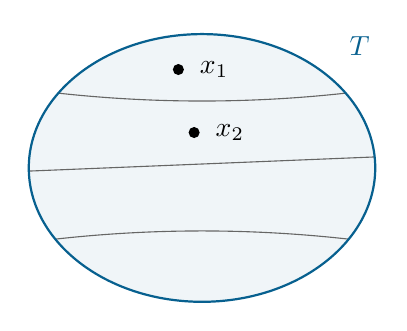
\begin{tikzpicture}
    % (1) Light fill of T
    \fill[figBlue!6] (0, 0) ellipse (2.2 and 1.7);

    % (2) Partition curves clipped inside T
    \begin{scope}
        \clip (0, 0) ellipse (2.2 and 1.7);
        \draw[figGray, domain=-2.2:2.2, samples=40, smooth] plot (\x, {0.85 + 0.03*\x*\x});
        \draw[figGray] (-2.2, -0.04) -- (2.2, 0.14);
        \draw[figGray, domain=-2.2:2.2, samples=40, smooth] plot (\x, {-0.80 - 0.03*\x*\x});
    \end{scope}

    % (3) Outline of T
    \draw[thick, figBlue] (0, 0) ellipse (2.2 and 1.7);

    % (4) Chosen orbit representatives
    \fill (-0.3, 1.25) circle (2pt);
    \fill (-0.1, 0.45) circle (2pt);

    % (5) Text last
    \node[anchor=west] at (-0.15, 1.25) {$x_1$};
    \node[anchor=west] at (0.05, 0.45) {$x_2$};
    \node[anchor=south west, figBlue] at (1.75, 1.30) {$T$};
\end{tikzpicture}
\end{center}

\begin{proposition}\label[proposition]{prop:orbit-decomposition}
If $G$ and $T$ are finite and $G \curvearrowright T$, then
\[
|T| = \sum_{E \in \text{Equiv.\ classes of } \sim} |E|
= \sum_{\substack{\text{choice of one } x \\ \text{per equiv.\ class}}} |\operatorname{Orb}(x)|
= \sum \left| \faktor{G}{\operatorname{Stab}(x)} \right|.
\]
\end{proposition}

\begin{steps}[Divisibility Constraint on Every Summand]
By \cref{cor:orbit-divides-group}, each summand $|\operatorname{Orb}(x)| = \left|\faktor{G}{\operatorname{Stab}(x)}\right|$ is a positive divisor of $|G|$. Thus, $|T|$ is expressed as a sum of divisors of $|G|$. In particular, the lecturer highlights the special orbit size $1$, whose formal definition is deferred to the next lecture.
\end{steps}

$\text{Def}\colon$ \inlinemetanote{video cuts off}
\end{content}

\begin{overview}[Summary of Key Concepts]
\begin{itemize}
    \item \textbf{The Symmetric Group $\operatorname{Sym}(T)$:} For $|T| = n$, $\operatorname{Sym}(T) \cong S_n$; for infinite $T$, $\operatorname{Sym}(T)$ is vastly larger (for instance, $\operatorname{Sym}(\mathbb{Z})$ is uncountable by encoding sequences in $\{0, 1\}^{\mathbb{N}}$ via disjoint swaps of $\{2k-1, 2k\}$), which is why later settings typically restrict to actions preserving extra structure on $T$.
    \item \textbf{Notation and Canonical Embeddings:} A group action $G \curvearrowright T$ corresponds equivalently to a map $\varphi \colon G \times T \to T$ or a homomorphism $\sigma \colon G \to \operatorname{Sym}(T)$ (stylistically written $\sigma_g(t)$). In \cref{thm:cayley-board}, saying a finite group $G$ \qt{is} a subgroup of $S_{|G|}$ expresses that $G$ is canonically isomorphic to a subgroup of $\operatorname{Sym}(G)$ via $G \curvearrowright G$.
    \item \textbf{Structure-Dependent Isomorphisms:} $\mathbb{R} \not\cong \mathbb{C}$ as rings (distinguished by $x^2 + 1 = 0$) and as $\mathbb{R}$-vector spaces ($\dim_{\mathbb{R}} \mathbb{R} = 1 \neq 2 = \dim_{\mathbb{R}} \mathbb{C}$), whereas $\mathbb{R} \cong \mathbb{C}$ as abelian groups.
    \item \textbf{Orbits and Stabilizers:} Any group action $G \curvearrowright T$ induces the equivalence relation $x \sim y \iff \exists g \in G \text{ s.t.\ } g \cdot x = y$ (\cref{def:orbit-equiv-rel,prop:orbit-is-equiv}), partitioning $T = \coprod E$ into $G$-invariant orbits $\operatorname{Orb}(x) = \{g \cdot x \mid g \in G\}$ (\cref{def:orbit,clm:orbit-g-invariant}). For each $x \in T$, the stabilizer $\operatorname{Stab}(x) = \{g \in G \mid g \cdot x = x\}$ is a subgroup of $G$ (\cref{def:stabilizer,lem:stab-is-subgroup}).
    \item \textbf{The Orbit--Stabilizer Theorem (\cref{thm:orbit-stabilizer}):} For any $G \curvearrowright T$ and $x \in T$, the map $C \colon \faktor{G}{\operatorname{Stab}(x)} \to \operatorname{Orb}(x)$ defined by $C\bigl(g \cdot \operatorname{Stab}(x)\bigr) = g \cdot x$ is a well-defined bijection satisfying $C \circ B = A$, where $B(g) = g \cdot \operatorname{Stab}(x)$ and $A(g) = g \cdot x$.
    \item \textbf{Finite Counting Consequences:} When $G$ is finite, every orbit $\operatorname{Orb}(x)$ is finite and $|\operatorname{Orb}(x)| = \left|\faktor{G}{\operatorname{Stab}(x)}\right|$ divides $|G|$ by Lagrange's Theorem (\cref{cor:orbit-divides-group}). When both $G$ and $T$ are finite, choosing one representative $x$ per equivalence class gives $|T| = \sum_x |\operatorname{Orb}(x)| = \sum_x \left|\faktor{G}{\operatorname{Stab}(x)}\right|$ (\cref{prop:orbit-decomposition}), expressing $|T|$ as a sum of divisors of $|G|$.
\end{itemize}
\end{overview}